\documentclass[journal]{IEEEtran}

\usepackage{cite}
\usepackage{amsmath,amssymb,amsfonts}
\usepackage{graphicx}
\usepackage{booktabs}
\usepackage{array}
\usepackage{url}
\usepackage{textcomp}
\usepackage{xcolor}
\usepackage{algorithm}
\usepackage{algorithmic}

\hyphenation{Aqua-Sim under-water event-triggered hold-time}

\begin{document}

\title{Event-Triggered Topology Discovery and Hold-Time-Aware Forwarding
for Mobile USV--AUV Acoustic Networks}

\author{Ghulam Ali%
\thanks{G.~Ali is the corresponding author (e-mail: ghulamali.cs@gmail.com).}%
}

\markboth{IEEE Internet of Things Journal}{Ali: Event-Triggered Discovery and Hold-Time-Aware Forwarding}

\maketitle

\begin{abstract}
Mobile unmanned-surface-vehicle (USV) and autonomous-underwater-vehicle (AUV)
teams must keep a usable acoustic topology while remaining inside a two-kilobit-per-second
control budget. Recent underwater routing studies, including Q-learning designs
such as LQARP, typically treat neighbor tables and link-quality estimates as
already accurate, or they score connectivity with a geometric range disc.
This paper treats topology discovery as the first object of study and then
forwards on the map that discovery actually produces.
We implement a sonar-equation link model---Thorp absorption, practical spreading,
Wenz noise, and a BPSK packet-success gate---on Aqua-Sim-NG in NS-3, and we let
HELLO beacons contend on unslotted ALOHA. An event-triggered send-on-delta
policy with an SNR-aware timeout is compared with periodic beaconing across
thirty randomized seeds. Event-triggered discovery at $T_{\max}=25$\,s reduces
control traffic from $927$\,bit/s to $212$\,bit/s (about $11\%$ of a $2$\,kbps
budget) while keeping precision at $0.994$; the cost is recall $0.841$ versus
$0.966$. On a relay-stable inner/outer field, the proposed ETHA protocol
(event-triggered HELLO, hold-time filter, and depth-primary next-hop scoring)
delivers packet delivery ratio $0.755\pm 0.031$ at $2.82$\,kJ, against
$0.641\pm 0.027$ at $4.61$\,kJ for periodic SNR-greedy forwarding
($n=30$, $12$ nodes, $95\%$ Student-$t$ intervals). The same event map with
SNR-greedy scoring reaches only $0.651$, so geography---not HELLO density---is
the first-order PDR lever once the table is good enough. An oracle with perfect
geometry reaches $0.817$, locating the residual in missing relays rather than
in hop scoring. The results argue for spending saved HELLO bits on a usable
map before importing reinforcement-learning routing.
\end{abstract}

\begin{IEEEkeywords}
Underwater acoustic networks, AUV, USV, topology discovery, event-triggered
control, link-quality estimation, hold time, ALOHA, Aqua-Sim-NG, NS-3.
\end{IEEEkeywords}

\noindent\textbf{Note to Practitioners:}
Ocean-IoT deployments that mix a USV sink with a small AUV team cannot
copy Wi-Fi HELLO intervals. At $1$\,kbps BPSK, a $50$-byte beacon every
$5$\,s already consumes half of a $2$\,kbps control budget once twelve
nodes share unslotted ALOHA. This paper gives operators a measured
trade. For topology awareness, event-triggered beacons at
$T_{\max}=25$\,s hold that budget to about $11\%$, at the cost of slower
link-up ($15$\,s) and a sparser neighbor table. For data delivery, spend
the saved bits on a shorter keep-alive ($T_{\max}=10$\,s) and a
depth-primary next hop toward the surface sink: ETHA then matches a
DBR-like baseline at $\mathrm{PDR}=0.755$ while cutting transmit energy
by about $39\%$ relative to periodic SNR-greedy HELLO. Hold-time filtering
stops dying relays; on a relay-stable field it rarely binds, and that
coincidence is reported rather than advertised as a PDR miracle.
The implementation is Aqua-Sim-NG/NS-3 and does not require sea-trial CSI
or a Bellhop field.

\section{Introduction}
\IEEEPARstart{U}{nderwater} acoustic links are slow, half-duplex, and
range-limited by absorption that grows with frequency
\cite{stojanovic2007capacity,stojanovic2009channels,urick1983sound}.
A surface craft acting as a sink for a team of AUVs therefore cannot
afford the HELLO rates that terrestrial mesh networks take for granted:
a $2$\,kbps-class control budget is already a large fraction of a
$1$\,kbps BPSK pipe \cite{liu2026lqarp,sozer2000uan,akyildiz2005uasn}.
At the same time the geometry is not static. Meandering currents and AUV
thrust move nodes across the decodable-range contour on a timescale of
tens of seconds \cite{caruso2008mcm}, so a neighbor table that is not
refreshed becomes both incomplete and stale.

Most underwater routing literature evaluates packet delivery ratio
(PDR) on a protocol that already assumes a neighborhood.
Vector-based forwarding (VBF) and depth-based routing (DBR) need
positions or depths \cite{xie2006vbf,yan2008dbr}.
QELAR and the more recent LQARP protocol learn next-hop Q-values from
rewards that mix energy, depth, and a link-quality term
\cite{hu2010qelar,liu2026lqarp}. Those designs are the right
\emph{second} chapter of a mobile USV--AUV network. They are the wrong
first chapter if the input map is a geometric disc, an offline Bellhop
table for moored nodes, or a HELLO process that has never been scored
against collisions and missed detections
\cite{casari2011protocol,chitre2008uwa,heidemann2012uwsns}.

This paper writes that first chapter. The question is mechanistic:
under a realistic acoustic budget, how should a mobile node spend
HELLO bits in order to know who is currently reachable, how good the
link is, and how long it will remain usable---and does that knowledge
change the next hop toward a USV sink? We answer it with a
simulation-only Aqua-Sim-NG/NS-3 campaign \cite{xie2009aquasim,aquasimng,ns3manual}
that is aligned with the acoustic stack of LQARP (source level, carrier,
Wenz shipping and wind, SNR threshold $8.68$\,dB, $400$-bit packets)
without copying its Q-learning router and without claiming a Bellhop
transmission-loss table we do not run.

The contributions are as follows.

\begin{enumerate}
\item \emph{A closed-form system model that matches the simulator.}
Section~\ref{sec:prelim} records the architecture, the Urick--Thorp--Wenz
channel, the multipath stand-in, and the Q-learning construction that
LQARP uses. Section~\ref{sec:model} then writes the graph, BPSK gate,
Caruso kinematics, unslotted ALOHA, and transmit energy as the
equations Aqua-Sim-NG actually integrates. A constant multipath margin
stands in for Bellhop; it is treated as a sensitivity parameter, not as
a ray trace.
\item \emph{Event-triggered, SNR-gated discovery under ALOHA.}
HELLO beacons contend in Aqua-Sim unslotted ALOHA. Decode uses the
sonar equation rather than a range disc. A send-on-delta policy in the
sense of event-triggered control \cite{tabuada2007event,heemels2012event}
is compared with periodic beaconing on thirty randomized seeds with
$95\%$ Student-$t$ confidence intervals.
\item \emph{ETHA: hold-time-aware forwarding on the discovered map.}
Each neighbor record carries an exponentially weighted moving average
(EWMA) of SNR \cite{woo2003taming} and a remaining useful time obtained
from radial opening speed and the SNR-threshold range $R^{\star}$.
The proposed next hop applies a hold-time filter and then a
depth-primary score toward the surface sink, using only neighbors the
node has actually heard.
\item \emph{A measured PDR and energy result, not a geometric claim.}
On twelve nodes with $T_{\max}=10$\,s, ETHA reaches
$\mathrm{PDR}=0.755\pm 0.031$ at $2.82$\,kJ and $480$\,bit/s of HELLO,
versus $0.641\pm 0.027$ at $4.61$\,kJ and $927$\,bit/s for periodic
SNR-greedy forwarding. An oracle bound of $0.817$ shows that the
remaining loss is missing relays. Q-learning the next hop would be
fitting the wrong residual.
\end{enumerate}

The rest of the paper is organized as LQARP is organized.
Section~\ref{sec:prelim} defines the network architecture, the
underwater acoustic propagation model, multipath as we treat it,
ambient noise, and the Q-learning technique.
Section~\ref{sec:related} locates prior protocols against that
background.
Section~\ref{sec:model} instantiates the channel in the simulator and
states mobility, MAC, energy, and the design problem.
Section~\ref{sec:proposed} presents event-triggered discovery and
hold-time-aware forwarding (ETHA).
Section~\ref{sec:eval} reports the Aqua-Sim campaign.
Section~\ref{sec:concl} concludes.

\section{Preliminaries}
\label{sec:prelim}

This section is definitional. It records the architecture of the
cell, the closed-form acoustics that every later equation uses, the
sense in which multipath is (and is not) present, the Wenz noise
field, and the Q-learning loop that QELAR and LQARP train
\cite{hu2010qelar,liu2026lqarp}.
No Q-table is estimated here, and no Bellhop eigenray is computed.
The empirical claims of the paper begin in
Section~\ref{sec:eval}; they are not smuggled into these definitions.

\subsection{Network Architecture}
\label{sec:arch}

A mobile ocean-IoT cell consists of one unmanned surface vehicle
(USV) and a small team of autonomous underwater vehicles (AUVs) that
share a single half-duplex acoustic carrier
\cite{akyildiz2005uasn,sozer2000uan}.
Index $0$ denotes the USV. It rides near the surface and is the unique
sink of every data packet. Indices $1,\ldots,N$ denote AUVs.
Nodes cannot transmit and receive at once, and they cannot occupy a
second frequency: control HELLO beacons and unicast DATA therefore
contend for the same $1$\,kbps BPSK pipe.

Fig.~\ref{fig:netarch} is the schematic.
The USV is a surface gateway with a downward-looking hydrophone.
AUVs occupy a water column whose depths, in this work, are drawn once
in $[40,160]$\,m and then held; the USV sits at $z=8$\,m.
Inner AUVs lie inside the SNR-threshold range of the USV and can act
as relays. Outer AUVs lie outside that range and require at least one
underwater hop.
Horizontal motion is the superposition of a meandering current
\cite{caruso2008mcm} and a bounded AUV thrust; the figure marks it
only as a drift.
HELLO is a one-hop broadcast. DATA is a unicast toward the USV.
There is no satellite backhaul in the model, no multi-USV backbone,
and no acoustic modem other than the Aqua-Sim-NG device used in
Section~\ref{sec:eval}.

The architecture is deliberately small.
Twelve nodes is already a crowded ALOHA neighborhood at $1$\,kbps
\cite{casari2011protocol}.
The schematic is not a fleet exercise. It makes the objects of
discovery and forwarding concrete before any protocol is written:
who can currently be heard, who can currently relay toward the
surface, and which of those facts a node is entitled to know.

\begin{figure*}[!t]
\centering
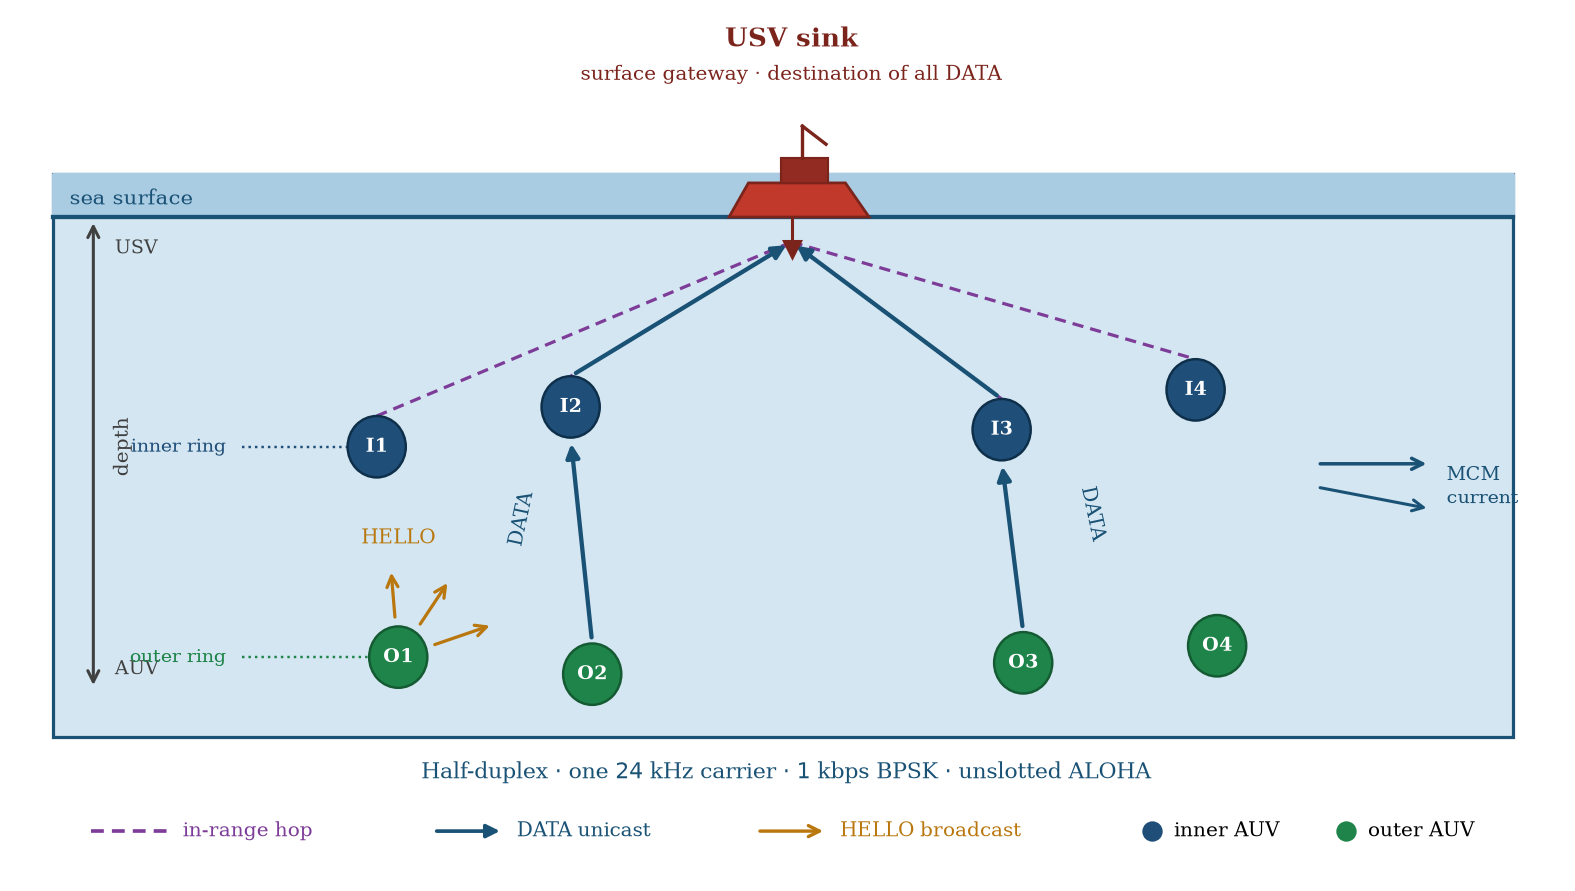
\includegraphics[width=0.98\textwidth]{figs/network_arch.png}
\caption{Schematic of the USV--AUV acoustic cell.
The USV is the unique sink. Inner AUVs (I1--I4) can reach it in one
hop; outer AUVs (O1--O4) require a relay.
Dashed purple segments are in-range acoustic hops; solid arrows are
DATA unicasts; orange arrows are a HELLO broadcast.
The drawing is a layout, not a measured snapshot.}
\label{fig:netarch}
\end{figure*}

\subsection{Underwater Acoustic Propagation Model}
\label{sec:prop}

Underwater links are slow, absorptive, and range-limited
\cite{stojanovic2007capacity,stojanovic2009channels,urick1983sound}.
The workhorse abstraction remains Urick's passive sonar equation
\cite{urick1983sound}
\begin{equation}
\gamma=\mathrm{SL}-\mathrm{TL}-\mathrm{NL}+\mathrm{DI}
\qquad\text{(dB),}
\label{eq:sonar}
\end{equation}
where $\mathrm{SL}$ is the source level, $\mathrm{TL}$ the
transmission loss, $\mathrm{NL}$ the noise level in the receiver
band, and $\mathrm{DI}$ the directivity index.
We take $\mathrm{SL}=185$\,dB re $1\,\mu\mathrm{Pa}$ at $1$\,m and
$\mathrm{DI}=0$\,dB, as in LQARP Table~II \cite{liu2026lqarp}.
The quantity $\gamma$ is an energy SNR. It is not a realized
channel impulse response.

Let $d$ be the Euclidean range in metres and $f$ the carrier in
kHz. Thorp's absorption, in dB/km, is
\cite{thorp1967attenuation,stojanovic2007capacity}
\begin{equation}
\alpha(f)=\frac{0.11f^{2}}{1+f^{2}}+\frac{44f^{2}}{4100+f^{2}}
+2.75\times 10^{-4}f^{2}+0.003.
\label{eq:thorp}
\end{equation}
Practical spreading with exponent $k=1.5$ interpolates between
spherical ($k=2$) and cylindrical ($k=1$) spreading
\cite{stojanovic2009channels}.
Together with a constant multipath margin $M$ defined in
Section~\ref{sec:multipath},
\begin{equation}
\mathrm{TL}(d)=10k\log_{10}d+\alpha(f)\,\frac{d}{1000}+M,
\qquad d\ge 1\,\mathrm{m}.
\label{eq:tl}
\end{equation}
Sound speed is held at $c=1500$\,m/s. There is no sound-speed
profile and no refraction. Propagation delay is $d/c$.

Substituting \eqref{eq:tl} into \eqref{eq:sonar} gives the
range-dependent SNR $\gamma(d)$.
A packet is declared decodable when
$\gamma(d)\ge\gamma_{\mathrm{th}}$ with
$\gamma_{\mathrm{th}}=8.68$\,dB \cite{liu2026lqarp}.
The unique range
\begin{equation}
R^{\star}=\arg_{d}\bigl\{\gamma(d)=\gamma_{\mathrm{th}}\bigr\}
\label{eq:rstar}
\end{equation}
is then well defined for each $(f,k,M,\mathrm{NL})$.
At the Table~II carrier $f_{c}=24$\,kHz and the operating margin
$M=30$\,dB used later, $R^{\star}=4946$\,m.
That number is a root of \eqref{eq:sonar}--\eqref{eq:tl}. It is not
a sea-trial measurement.

\subsection{Multipath Effects}
\label{sec:multipath}

A shallow waveguide does not deliver one arrival.
A transmitted pulse reaches the hydrophone as a sum of eigenrays
with different delays, amplitudes, and Doppler shifts
\cite{preisig2007propagation,vanwalree2013scattering}.
Two consequences matter for a $400$-bit packet at $1$\,kbps.

First, inter-symbol interference.
The symbol duration is $1$\,ms. A delay spread of tens of
milliseconds, which Preisig and van~Walree document as routine in
littoral channels, spans many symbols.
An energy SNR that ignores that spread overstates packet success.

Second, coherent fading.
The same rays can cancel at the hydrophone even when the
energy-based $\mathrm{TL}$ of \eqref{eq:tl} predicts a usable
$\gamma$. A node that sits inside $R^{\star}$ can still fail to
decode; a node that sits outside $R^{\star}$ can, rarely, succeed.
Equation~\eqref{eq:rstar} is a contour, not a wall.

Bellhop ray tracing is the standard way to import that structure
into a network simulator \cite{porter2011bellhop}.
LQARP does so for \emph{moored, static} nodes \cite{liu2026lqarp}.
This paper does not.
A mobile USV--AUV geometry would require a new ray trace at every
HELLO, which we do not compute, and an offline TL table computed on
a rest geometry is not a time-varying waveguide.
The only multipath object in the model is the constant margin $M$
in \eqref{eq:tl}.
It shortens $R^{\star}$ and stands in for unmodeled coherent loss.
It is not a delay-spread process, not a tap filter, and not a
substitute for sea-trial CSI.
Section~\ref{sec:eval} sweeps $M\in\{20,30,40\}$\,dB as a
sensitivity check: because nodes are placed as fractions of
$R^{\star}$, discovery recall does not move in any operationally
meaningful way.
That is a statement about placement, not a claim that multipath is
harmless.

\subsection{Ambient Noise}
\label{sec:noise}

Ambient noise in the band of interest is the four-component Wenz
model, in dB re $1\,\mu\mathrm{Pa}/\mathrm{Hz}$
\cite{wenz1962noise,stojanovic2009channels,liu2026lqarp}:
\begin{subequations}
\label{eq:wenz}
\begin{align}
N_{\mathrm{t}}(f)&=17-30\log_{10}f,\\
N_{\mathrm{s}}(f)&=40+20(s-0.5)+26\log_{10}f \nonumber\\
&\quad-60\log_{10}(f+0.03),\\
N_{\mathrm{w}}(f)&=50+7.5\sqrt{w}+20\log_{10}f \nonumber\\
&\quad-40\log_{10}(f+0.4),\\
N_{\mathrm{th}}(f)&=-15+20\log_{10}f.
\end{align}
\end{subequations}
The four terms are turbulence, shipping, wind-driven wave noise, and
thermal noise.
Shipping activity $s=0.2$ and wind speed $w=2$\,m/s are taken from
LQARP Table~II.
The noise level in a band of width $B$\,Hz is obtained by converting
each component to linear units and summing,
\begin{equation}
\mathrm{NL}=10\log_{10}\!\left(B\sum_{x\in\{\mathrm{t,s,w,th}\}}10^{N_x(f)/10}\right).
\label{eq:nl}
\end{equation}
Equation~\eqref{eq:nl} is spatially homogeneous and temporally
white in the packet band.
There is no shipping-lane map, no rain term, no measured PSD, and
no site-specific Wenz fit.
It is the only noise the simulator uses, and it is the $\mathrm{NL}$
that enters \eqref{eq:sonar}.

\subsection{Q-learning Technique}
\label{sec:qlearn}

Q-learning is a model-free method for estimating the action-value
function of a Markov decision process
\cite{watkins1992qlearning,sutton2018rl}.
An agent in state $s$ selects action $a$, receives a scalar reward
$r$, and observes a successor $s'$.
With learning rate $\alpha_Q\in(0,1]$ and discount
$\eta\in[0,1)$---we write $\eta$ rather than the usual $\gamma$, and
$\alpha_Q$ rather than $\alpha$, to avoid collision with SNR and with
Thorp absorption---the Watkins update is
\begin{equation}
Q(s,a)\leftarrow
(1-\alpha_Q)\,Q(s,a)
+\alpha_Q\Bigl[r+\eta\max_{a'}Q(s',a')\Bigr].
\label{eq:qupdate}
\end{equation}
A greedy policy reads
$\pi(s)=\arg\max_{a}Q(s,a)$.
Fig.~\ref{fig:qlearn} is that loop, drawn as a routing agent.

In underwater next-hop routing the natural identification is
\cite{hu2010qelar,liu2026lqarp}
\begin{equation}
s=i,\qquad
a=j\in\widehat{\mathcal{N}}_{i}(t),\qquad
s'=j,
\label{eq:qmap}
\end{equation}
where $i$ is the current holder of the packet and $j$ is a neighbor
the node has actually heard.
The reward is protocol-specific.
QELAR places residual energy in $r$ \cite{hu2010qelar}.
LQARP adds an explicit link-quality term derived from the sonar
equation, together with a depth term toward the sink
\cite{liu2026lqarp}.
A generic form that covers both, without inventing coefficients
those papers use and we have not re-estimated, is
\begin{equation}
r(s,a)=
\beta_{\mathrm{LQ}}\,r_{\mathrm{LQ}}
+\beta_{\mathrm{z}}\,r_{\mathrm{z}}
+\beta_{\mathrm{E}}\,r_{\mathrm{E}},
\label{eq:qrew}
\end{equation}
with $r_{\mathrm{LQ}}$ increasing in SNR,
$r_{\mathrm{z}}$ increasing as the next hop shallows toward the
USV, and $r_{\mathrm{E}}$ increasing in residual energy.
The weights $(\beta_{\mathrm{LQ}},\beta_{\mathrm{z}},\beta_{\mathrm{E}})$
belong to the protocol that trains \eqref{eq:qupdate}.
They are not fitted in this paper.

Two structural facts follow from \eqref{eq:qmap} and are the reason
this subsection exists.

First, the action set is the neighbor table.
If $j$ has never been heard, $Q(i,j)$ is not an entry that
\eqref{eq:qupdate} is entitled to update.
A learner trained on a geometric disc, or on an offline Bellhop
table for moored nodes, is solving a different MDP than a mobile
node whose table is an ALOHA process.

Second, greedy Q-learning, like greedy geographic routing, can
stall in a \emph{void}: a local minimum of the progress function
from which every available next hop fails to approach the sink
\cite{noh2013vapr,coutinho2014gedar,yan2008dbr}.
Write
\begin{equation}
\mathcal{P}_{i}(t)=
\bigl\{j\in\widehat{\mathcal{N}}_{i}(t):
\mathrm{prog}(j,0)>\mathrm{prog}(i,0)\bigr\}
\label{eq:progress}
\end{equation}
for the progress set, with $\mathrm{prog}(\cdot,0)$ a decreasing
function of depth or of range to the USV.
Node $i$ is in a local void when $\mathcal{P}_{i}(t)=\emptyset$
while a path from $i$ to the sink still exists in the true graph.
Fig.~\ref{fig:void} is that geometry.
The greedy hop (dotted) points at a shallower node that is
\emph{not} a neighbor.
The available neighbors (green) do not reduce depth or range.
A detour through a non-greedy neighbor $k$ can restore progress;
LQARP's void handling is of that kind \cite{liu2026lqarp}.
A network partition is a different object: if no path exists, no
detour exists either.

This paper does not train \eqref{eq:qupdate} and does not run a
void-recovery campaign.
ETHA's next hop, defined in Section~\ref{sec:proposed}, is a
score on the live table, not a learned $Q$.
The oracle bound in Section~\ref{sec:eval} has zero no-route on the
relay-stable field, which means that field is not a void field:
the residual is missing table entries, not a local minimum of
depth.
Q-learning remains the intended sequel once that residual is the
one that remains, and only among neighbors the node has actually
heard.

\begin{figure*}[!t]
\centering
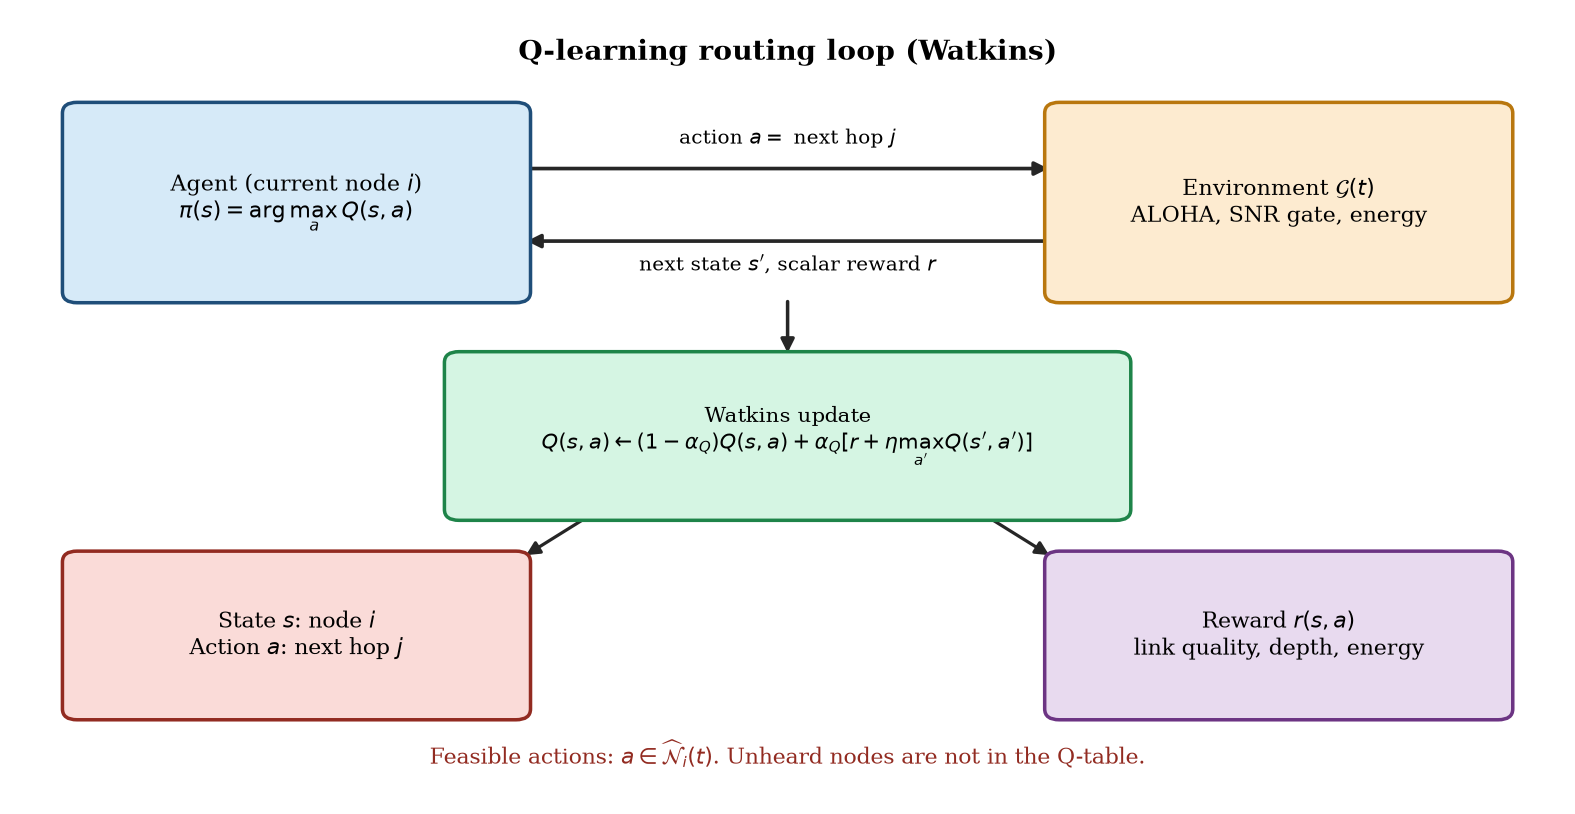
\includegraphics[width=0.98\textwidth]{figs/qlearning.png}
\caption{Q-learning framework for next-hop routing
(Watkins update \eqref{eq:qupdate}).
The agent is the current holder of the packet; the environment is
the acoustic network; the action is a next hop.
Feasible actions are heard neighbors only.
This figure is the loop trained by QELAR and LQARP. It is not a
loop trained in this paper.}
\label{fig:qlearn}
\end{figure*}

\begin{figure}[!t]
\centering
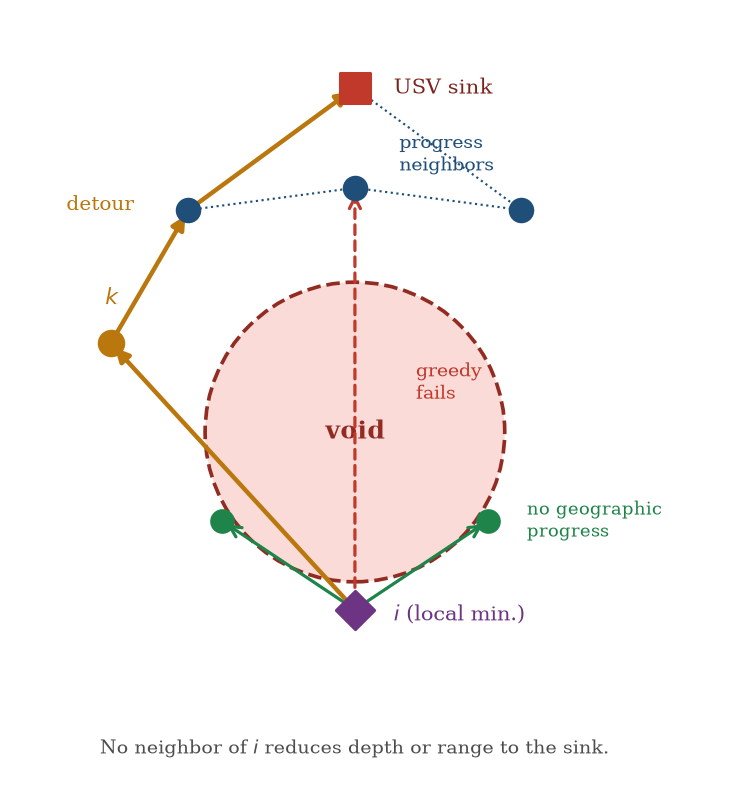
\includegraphics[width=0.92\columnwidth]{figs/void_area.png}
\caption{Schematic of a geographic void.
Node $i$ is a local minimum: its heard neighbors do not reduce
depth or range to the USV, so a greedy progress rule fails.
A non-greedy neighbor $k$ restores a path.
The drawing is pedagogical. It is not a layout from the Aqua-Sim
campaign, and no void-recovery PDR is reported.}
\label{fig:void}
\end{figure}

\section{Related Work}
\label{sec:related}

Section~\ref{sec:prelim} defined the acoustic primitives.
This section locates prior protocols relative to them.

\subsection{Acoustic Channels and Link Abstraction}
The sonar equation, Thorp absorption, practical spreading, and Wenz
noise of Section~\ref{sec:prop}--\ref{sec:noise} are standard
\cite{urick1983sound,thorp1967attenuation,wenz1962noise,stojanovic2007capacity,stojanovic2009channels}.
Preisig and van~Walree emphasize that real waveguides add coherent
multipath and scattering that no $k$-spreading law captures
\cite{preisig2007propagation,vanwalree2013scattering}.
Bellhop ray tracing is the standard way to import that structure
\cite{porter2011bellhop}. LQARP uses an offline Bellhop table for
\emph{static} moored nodes \cite{liu2026lqarp}. We do not. The constant
margin $M$ of Section~\ref{sec:multipath} is the only multipath object
in the simulator, and Section~\ref{sec:eval} treats it as a sensitivity
parameter, not as a ray trace.

\subsection{Topology Discovery and Link-Quality Estimation}
Terrestrial sensor nets learned that neighborhood is a measurement
problem: EWMA of packet success, four-bit estimators, and hysteresis
on SNR \cite{woo2003taming,fonseca2007fourbit}. Underwater, the same
need is sharper because a HELLO occupies hundreds of milliseconds and
a collision wastes a long propagation slot
\cite{casari2011protocol,chitre2008uwa,akyildiz2007state}.
Periodic HELLO is the default in Aqua-Sim examples and in most routing
evaluations \cite{xie2009aquasim}. Event-triggered and self-triggered
control replace periodic sampling with a send-on-delta rule that
guarantees a minimum inter-event time $T_{\min}$ and a keep-alive
$T_{\max}$ \cite{tabuada2007event,heemels2012event}.
We import that structure to acoustic HELLOs and score it against
ground-truth SNR-gated edges, not against PDR of a router that hides
the table.

\subsection{Geographic and Opportunistic Forwarding}
VBF forwards inside a routing pipe toward the sink \cite{xie2006vbf};
HH-VBF rebuilds the pipe per hop \cite{nicolaou2007hhvbf};
DBR and VAPR use depth or pressure and void awareness
\cite{yan2008dbr,noh2013vapr};
GEDAR adds depth adjustment \cite{coutinho2014gedar}.
All of them need a current neighbor set. None of them is the
experiment in this paper. We use geographic progress and a DBR-like
depth score only so that discovery quality is visible in PDR, energy,
stale hops, and no-route drops.

\subsection{Learning Routers}
QELAR treats forwarding as a distributed MDP with residual energy in
the reward \cite{hu2010qelar}. LQARP adds an explicit link-quality
term derived from the sonar equation and evaluates Q-learning next-hop
selection on a static UWSN with ALOHA and a Bellhop TL table
\cite{liu2026lqarp}.
Section~\ref{sec:qlearn} recorded that loop without training it.
Those papers are the baseline we follow for
\emph{parameters} (Table~II of LQARP) and for the intended venue.
They are not the algorithm we run. Table~\ref{tab:vs} states the
difference in one place. Importing Q-learning onto a map
whose event-triggered recall is $0.84$ would attribute discovery loss
to the learner. Section~\ref{sec:eval} makes that residual explicit.

\begin{table}[!t]
\caption{Position Relative to Closely Related Protocols}
\label{tab:vs}
\centering
\setlength{\tabcolsep}{2.4pt}
\resizebox{\columnwidth}{!}{%
\begin{tabular}{lcccc}
\toprule
 & DBR & QELAR & LQARP & ETHA \\
\midrule
HELLO process scored & no & no & no & \textbf{yes} \\
Event-triggered beacons & no & no & no & \textbf{yes} \\
SNR-gated decode & range & energy MDP & sonar+Bellhop & sonar, no Bellhop \\
Hold-time feature & no & no & no & \textbf{yes} \\
Depth toward sink & yes & reward & reward & depth-primary \\
Q-learning & no & yes & yes & no (future) \\
Mobility in evaluation & limited & static energy & static UWSN & MCM+AUV thrust \\
\bottomrule
\end{tabular}}
\end{table}

\section{System Model}
\label{sec:model}

This section instantiates Section~\ref{sec:prelim} as the objects
Aqua-Sim-NG integrates: the time-varying graph, the pairwise SNR,
the BPSK erasure, Caruso kinematics, unslotted ALOHA, and transmit
energy.
Notation follows LQARP's acoustic stack \cite{liu2026lqarp}.
The development remains analytical: there is no Bellhop field and no
sea-trial CSI. Table~\ref{tab:notation} lists the principal symbols.

\begin{table}[!t]
\caption{Principal Notation}
\label{tab:notation}
\centering
\setlength{\tabcolsep}{3.5pt}
\begin{tabular}{ll}
\toprule
Symbol & Meaning \\
\midrule
$\mathcal{V}$, $N$ & Node set; number of AUVs \\
$\mathcal{G}(t)$ & True SNR-gated directed graph at time $t$ \\
$\widehat{\mathcal{N}}_i(t)$ & Neighbor table of node $i$ \\
$d_{ij}$, $p_i$, $v_i$ & Range (m); position; velocity \\
$\alpha(f)$, $k$, $M$ & Thorp absorption; spreading; multipath margin \\
$\mathrm{SL}$, $\mathrm{TL}$, $\mathrm{NL}$, $\mathrm{DI}$ & Sonar-equation terms (dB) \\
$\gamma_{ij}$, $\gamma_{\mathrm{th}}$ & Instantaneous SNR; decode threshold \\
$R^{\star}$ & Range at which $\gamma=\gamma_{\mathrm{th}}$ \\
$p_{\mathrm{e}}$, $P_{\mathrm{succ}}$ & BPSK BER; packet success probability \\
$v_r$, $f_d$ & Radial relative speed; Doppler (Hz) \\
$T_{\min}$, $T_{\max}$ & Event-triggered inter-HELLO bounds \\
$\bar{s}_{ij}$, $H_{ij}$ & EWMA SNR; predicted hold (s) \\
$O_c$, $E_{\mathrm{tx}}$ & Control rate (bit/s); transmit energy (J) \\
$Q(s,a)$, $\alpha_Q$, $\eta$ & Action value; learning rate; discount \\
$\mathcal{P}_i(t)$ & Progress-neighbor set of node $i$ \\
\bottomrule
\end{tabular}
\end{table}

\subsection{Network Model}
Consider a set $\mathcal{V}=\{0,1,\ldots,N\}$ of half-duplex acoustic
nodes with the architecture of Fig.~\ref{fig:netarch}.
Index $0$ is the USV sink; indices $1,\ldots,N$ are AUVs.
A directed pair $(i,j)\in\mathcal{V}\times\mathcal{V}$, $i\neq j$,
is a \emph{true link} at time $t$ if and only if the pairwise SNR
of Section~\ref{sec:prop} satisfies
$\gamma_{ij}(t)\ge\gamma_{\mathrm{th}}$.
The true graph is
\begin{equation}
\mathcal{G}(t)=\bigl(\mathcal{V},\,\bigl\{(i,j):i\neq j,\;\gamma_{ij}(t)\ge\gamma_{\mathrm{th}}\bigr\}\bigr).
\label{eq:graph}
\end{equation}
Each node $i$ maintains a neighbor table $\widehat{\mathcal{N}}_i(t)$
from HELLO receptions. Discovery quality is the agreement between
$\widehat{\mathcal{N}}_i(t)$ and the true neighborhood of $i$ in
$\mathcal{G}(t)$. Data packets originated by AUVs have destination $0$.
Nodes share a single carrier and cannot transmit and receive at once.

Fig.~\ref{fig:scenario} shows the inner/outer placement used for
forwarding. Inner AUVs lie in $[0.62,0.82]R^{\star}$ and remain usable
relays. Outer AUVs lie in $[1.02,1.10]R^{\star}$ and require two hops.
A separate discovery layout places both rings on the $R^{\star}$
contour so that links form and break within $240$\,s.

\begin{figure}[!t]
\centering
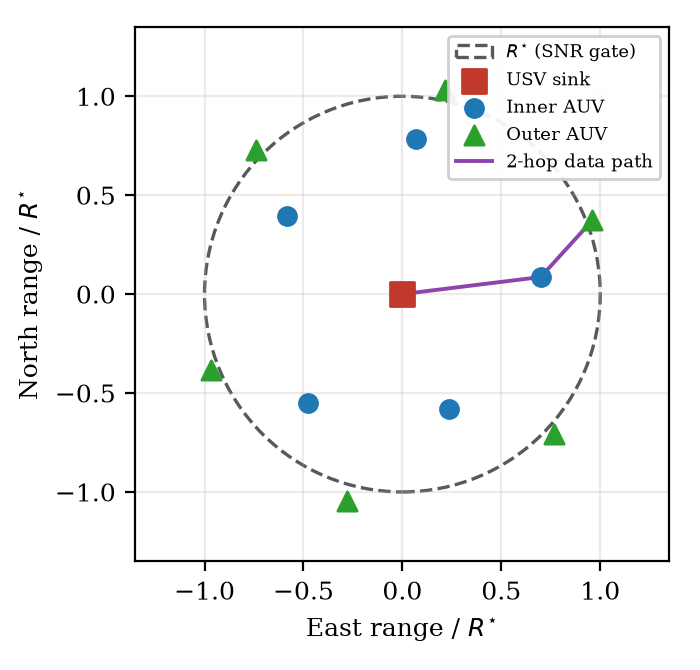
\includegraphics[width=0.92\columnwidth]{figs/scenario.png}
\caption{Inner/outer forwarding layout. Ranges are normalized by the
SNR-threshold range $R^{\star}$. Outer AUVs need a two-hop path through
the inner ring to the USV sink.}
\label{fig:scenario}
\end{figure}

\subsection{Acoustic Channel Instantiation}
The simulator integrates \eqref{eq:sonar}--\eqref{eq:nl} at
$f_{c}=24$\,kHz with the Table~II constants of
Section~\ref{sec:prop}--\ref{sec:noise}.
Let $d_{ij}(t)=\|p_i(t)-p_j(t)\|_2$. The pairwise SNR is
\begin{equation}
\gamma_{ij}(t)=\mathrm{SL}-\mathrm{TL}\bigl(d_{ij}(t)\bigr)-\mathrm{NL}+\mathrm{DI},
\label{eq:snr}
\end{equation}
and a packet is \emph{decodable} when
$\gamma_{ij}(t)\ge\gamma_{\mathrm{th}}$.
The range derivative used by the hold-time predictor is
\begin{equation}
\frac{\partial\mathrm{TL}}{\partial d}=\frac{10k}{d\ln 10}+\frac{\alpha(f)}{1000}
\qquad\text{(dB/m).}
\label{eq:dtl}
\end{equation}
Aqua-Sim's geometric transmit range is set to $1.35R^{\star}$ so that
the MAC can deliver a waveform that the SNR gate subsequently
rejects; those events are logged, not counted as neighbors.
Fig.~\ref{fig:channel} plots \eqref{eq:thorp}--\eqref{eq:psucc} at the
operating point: absorption, Wenz components, TL for three values of
$M$, and SNR together with $P_{\mathrm{succ}}$.
$P_{\mathrm{succ}}$ collapses in a few hundred metres around
$R^{\star}$; that cliff is the decode gate used in every experiment.

\begin{figure*}[!t]
\centering
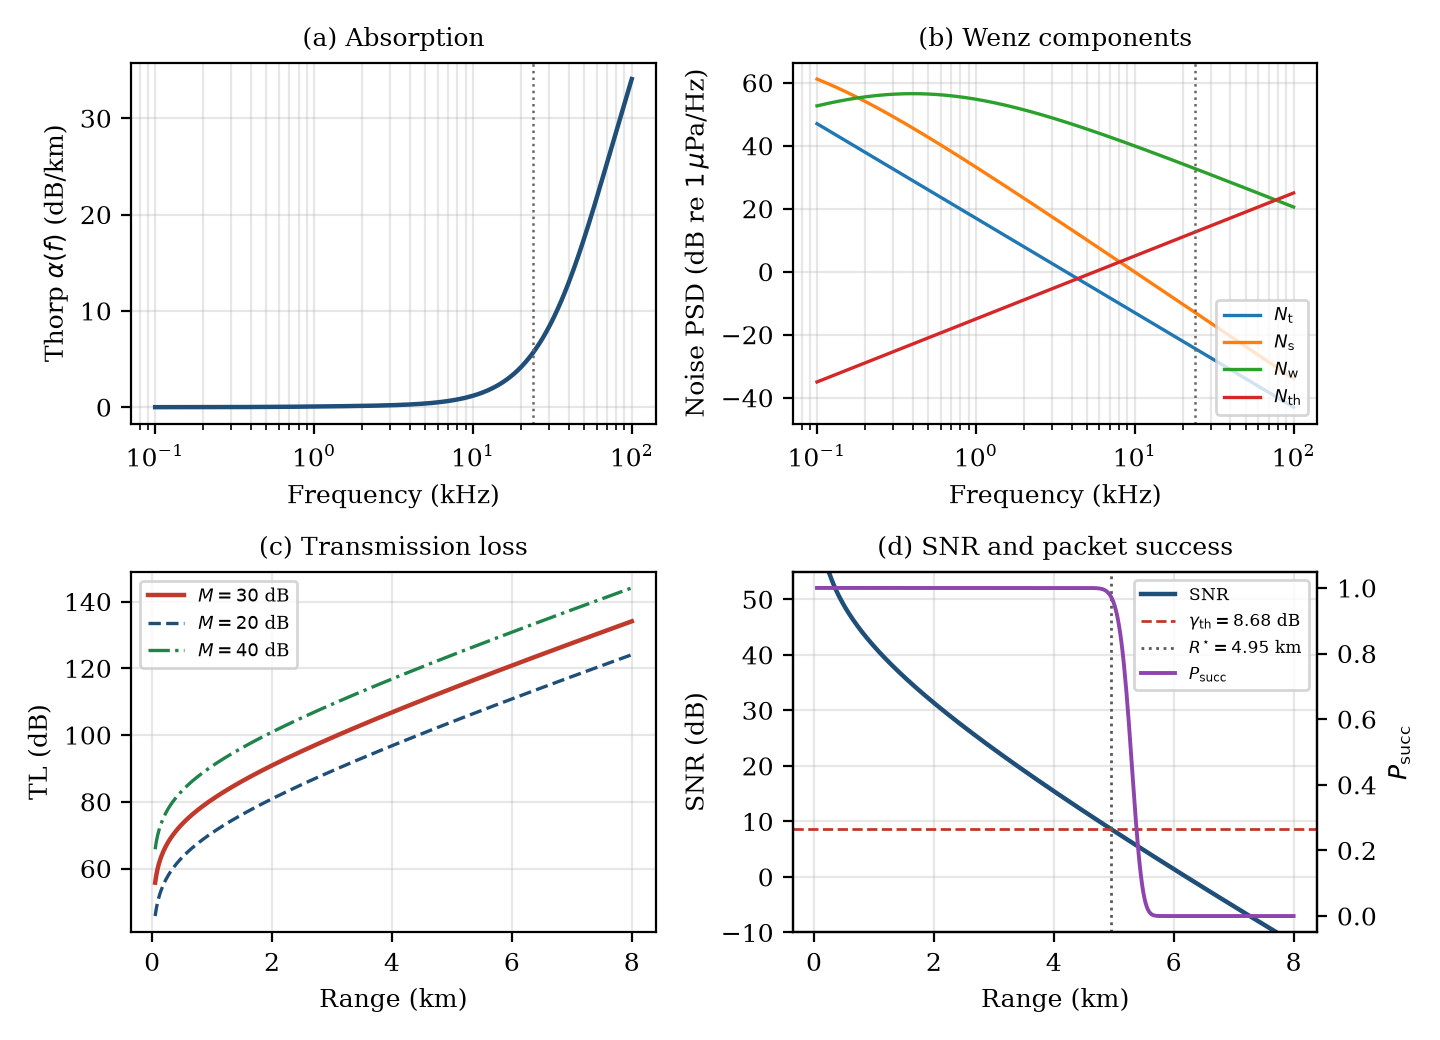
\includegraphics[width=0.98\textwidth]{figs/channel.png}
\caption{Closed-form acoustic stack used by the simulator (LQARP Table~II
parameters, $f_c=24$\,kHz, $k=1.5$, $s=0.2$, $w=2$\,m/s, $M=30$\,dB
unless swept). (a)~Thorp absorption. (b)~Wenz noise PSD components.
(c)~Transmission loss. (d)~SNR and BPSK packet success versus range,
with the SNR threshold $\gamma_{\mathrm{th}}$ and $R^{\star}$.
This is not Bellhop.}
\label{fig:channel}
\end{figure*}

\subsection{Packet-Error Model}
After ALOHA has delivered a waveform, BPSK bit errors follow LQARP
eqs.~(36)--(38) with constellation size $M=2$ \cite{liu2026lqarp}:
\begin{equation}
p_{\mathrm{e}}(\gamma)=\frac{1}{2}\,\mathrm{erfc}\sqrt{10^{\gamma/10}}.
\label{eq:pe}
\end{equation}
An $L$-bit packet succeeds with probability
\begin{equation}
P_{\mathrm{succ}}(\gamma)=\bigl(1-p_{\mathrm{e}}(\gamma)\bigr)^{L},\qquad L=400,
\label{eq:psucc}
\end{equation}
and is erased independently with probability $1-P_{\mathrm{succ}}$.
The same gate is applied to HELLO and to unicast data, so a next hop
that is already below $\gamma_{\mathrm{th}}$ cannot contribute to PDR.
Acoustic Doppler
\begin{equation}
f_{d}=f_{c}v_{r}/c,\qquad
v_{r}=\frac{(p_j-p_i)^{\top}(v_j-v_i)}{d_{ij}},
\label{eq:doppler}
\end{equation}
with $c=1500$\,m/s, is logged from the radial relative speed and is
not used as an additional decode threshold.

\subsection{Mobility Model}
Horizontal drift follows the meandering-current model (MCM) of Caruso
\emph{et al.} \cite{caruso2008mcm}. With wavelength $\lambda$,
nondimensional coordinates $x'=x/\lambda$, $y'=y/\lambda$, meander
amplitude $B'(t)=(B/\lambda)(1+\varepsilon\cos\omega t)$, and
$k_{\psi}=2\pi$, the stream function is
\begin{equation}
\psi(x',y',t)=-\tanh\!\left(\frac{y'-B'(t)\sin(k_{\psi}x')}{\sqrt{1+k_{\psi}^{2}B'(t)^{2}\cos^{2}(k_{\psi}x')}}\right).
\label{eq:psi}
\end{equation}
The current is $u=U_0\partial\psi/\partial y'$,
$v=-U_0\partial\psi/\partial x'$
with $U_0$ drawn per seed in $[0.30,0.60]$\,m/s. Each AUV $i$ adds a
bounded thrust $u_i^{\mathrm{th}}$, so
\begin{equation}
\dot{p}_i(t)=\bigl(u(p_i,t),\,v(p_i,t)\bigr)+u_i^{\mathrm{th}}.
\label{eq:pdot}
\end{equation}
Depth is drawn once in $[40,160]$\,m for AUVs and held; the USV sits
at $z=8$\,m. This is kinematics, not an ocean general circulation
model and not a vehicle autopilot.

\subsection{MAC and Energy Consumption}
Nodes share unslotted ALOHA with $\mathrm{AckOn}=0$ at bit rate
$R_b=1000$\,bit/s \cite{aquasimng,liu2026lqarp}. Packet duration is
\begin{equation}
T_{\mathrm{tx}}=L/R_b=0.4\,\mathrm{s}.
\label{eq:ttx}
\end{equation}
Propagation at $R^{\star}$ is $T_{\mathrm{prop}}=R^{\star}/c\approx 3.3$\,s,
so a one-hop flight is about $3.7$\,s. Transmit energy for
$N_{\mathrm{tx}}$ packets (HELLO plus data originations and forwards)
at electrical power $P_T=10$\,W is
\begin{equation}
E_{\mathrm{tx}}=P_T T_{\mathrm{tx}} N_{\mathrm{tx}}=4N_{\mathrm{tx}}\quad\text{(joules).}
\label{eq:energy}
\end{equation}
Receive power is not an independent Aqua-Sim-NG parameter in this
build; reported energy is therefore transmit energy only.
Control rate against a $2$\,kbps reference budget is
\begin{equation}
O_{c}=\frac{N_{\mathrm{HELLO}}L}{T_{\mathrm{sim}}}.
\label{eq:oh}
\end{equation}
A slotted-ALOHA control with slot
$T_{\mathrm{tx}}+T_{\mathrm{prop,max}}+\mathrm{guard}\approx 5.06$\,s
is reported as a negative result in discovery: the slot synchronizes
the $5$\,s HELLO period and \emph{raises} collisions.

\subsection{Problem Statement}
Over a horizon $[0,T_{\mathrm{sim}}]$, each node must choose HELLO
instants and, on each data packet, a next hop
$j\in\widehat{\mathcal{N}}_i(t)\cup\{\emptyset\}$.
Writing $\pi_{\mathrm{HELLO}}$ for the beacon policy and
$\pi_{\mathrm{hop}}$ for the hop rule, the design problem is
\begin{equation}
\begin{aligned}
\max_{\pi_{\mathrm{HELLO}},\,\pi_{\mathrm{hop}}}\quad
&\mathbb{E}\bigl[\mathrm{PDR}\bigr] \\
\mathrm{s.t.}\quad
& O_c\le 2\,\mathrm{kbps}, \\
& j\in\widehat{\mathcal{N}}_i(t)\cup\{\emptyset\},
\end{aligned}
\label{eq:opt}
\end{equation}
where the expectation is over seeds (placement, current, ALOHA, BPSK).
We do not solve \eqref{eq:opt} as a global MDP. We specify an
event-triggered HELLO rule and a hold-time-aware hop filter, then
measure the resulting discovery and delivery residuals against
periodic HELLO, SNR-greedy forwarding, a DBR-like depth rule, and an
oracle with perfect geometry.

\section{Proposed ETHA Protocol}
\label{sec:proposed}

ETHA (event-triggered hold-time-aware discovery and forwarding)
has four parts: the neighbor record, the HELLO policy, the hold-time
predictor, and the next-hop rule. Fig.~\ref{fig:protocol} is the
architecture; Fig.~\ref{fig:scenario} is the topology on which the hop
rule is evaluated; discovery is evaluated on the contour-crossing
layout of Section~\ref{sec:eval}.

\begin{figure*}[!t]
\centering
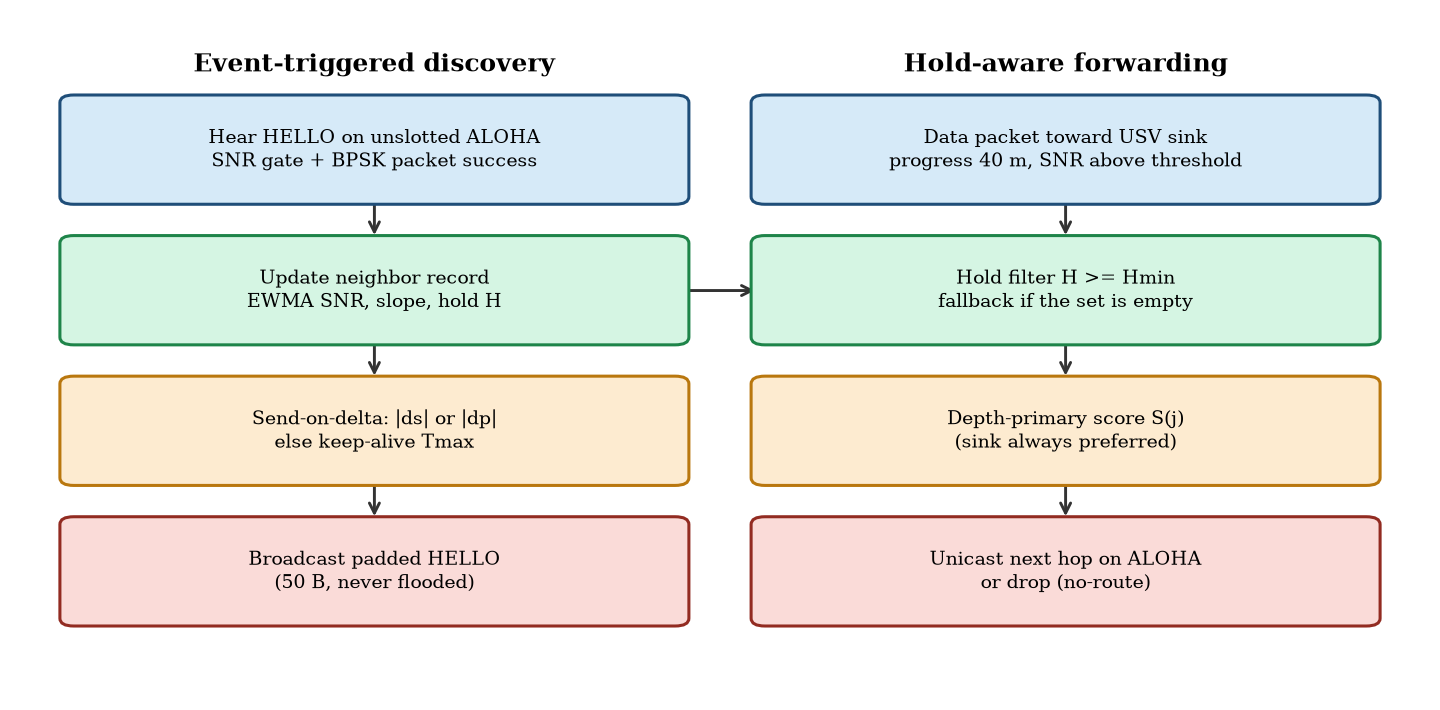
\includegraphics[width=0.98\textwidth]{figs/protocol.png}
\caption{ETHA architecture. Left: event-triggered, SNR-gated HELLO on
unslotted ALOHA. Right: hold-time filter and depth-primary next hop
toward the USV, using only neighbors the node has actually heard.}
\label{fig:protocol}
\end{figure*}

\subsection{Neighbor Record and EWMA Link Quality}
When $i$ decodes a HELLO from $j$, it stores last range, velocity,
and SNR $s_{ij}$. Link quality is the EWMA
\cite{woo2003taming}
\begin{equation}
\bar{s}_{ij}(t)=\lambda s_{ij}(t)+(1-\lambda)\bar{s}_{ij}(t^{-}),\qquad\lambda=0.35,
\label{eq:ewma}
\end{equation}
with slope
$\dot{\bar{s}}_{ij}=(\bar{s}_{ij}(t)-\bar{s}_{ij}(t^{-}))/\Delta t$.
Neighbor $j$ remains in $\widehat{\mathcal{N}}_i(t)$ while
$t-t_{ij}^{\mathrm{rx}}$ is within a timeout
\begin{equation}
\tau_{ij}=\min\bigl\{\tau_{\mathrm{base}},\,\max(5,H_{ij}+4),\,\tau_{\mathrm{fade}}\bigr\},
\label{eq:timeout}
\end{equation}
where $\tau_{\mathrm{base}}=3T$ (periodic) or $2T_{\max}$ (event),
$H_{ij}$ is the predicted hold, and $\tau_{\mathrm{fade}}=8$\,s if
$\bar{s}_{ij}<\gamma_{\mathrm{th}}+3$\,dB with negative slope.
Equation~\eqref{eq:timeout} is why link-down delay does not track
$T_{\max}$.

\subsection{Event-Triggered HELLO}
Periodic mode emits a HELLO every $T=5$\,s plus a few hundred
milliseconds of jitter.

Event-triggered mode is send-on-delta
\cite{tabuada2007event,heemels2012event}. Let $t_{\ell}$ be the last
transmission, $p_{\ell}$ the position then, and $s_{\ell}$ the SNR
to the USV then. A HELLO is eligible only if $t-t_{\ell}\ge T_{\min}$
($T_{\min}=5$\,s) and is forced if $t-t_{\ell}\ge T_{\max}$. Between
those bounds $i$ transmits when
\begin{equation}
\bigl|s_{\mathrm{USV}}(t)-s_{\ell}\bigr|\ge\Delta_{s}
\quad\text{or}\quad
\|p_i(t)-p_{\ell}\|\ge\Delta_{p},
\label{eq:delta}
\end{equation}
with $\Delta_{s}=4$\,dB and $\Delta_{p}=150$\,m
(Algorithm~\ref{alg:hello}). Outer nodes whose USV SNR is already
below $\gamma_{\mathrm{th}}$ do not treat a dead USV link as a
permanent event; they fall back to $T_{\max}$ so the ring does not
beacon every $T_{\min}$.

HELLOs carry identity, position, and velocity ($28$\,bytes) and are
padded to $50$\,bytes. They are sent through the Aqua-Sim device so
ALOHA collisions are real. They are never flooded.

\begin{algorithm}[!t]
\caption{Event-triggered HELLO at node $i$}
\label{alg:hello}
\begin{algorithmic}[1]
\STATE $t_{\ell}\leftarrow -\infty$, $p_{\ell}\leftarrow p_{i}$, $s_{\ell}\leftarrow -\infty$
\LOOP
\STATE wait until $t-t_{\ell}\ge T_{\min}$
\STATE $s\leftarrow$ SNR to USV; $\Delta p\leftarrow \|p_{i}-p_{\ell}\|$
\IF{$t-t_{\ell}\ge T_{\max}$ \textbf{or} ($s\ge\gamma_{\mathrm{th}}$ \textbf{and} ($|s-s_{\ell}|\ge\Delta_{s}$ \textbf{or} $\Delta p\ge\Delta_{p}$))}
\STATE broadcast padded HELLO on ALOHA
\STATE $t_{\ell}\leftarrow t$, $p_{\ell}\leftarrow p_{i}$, $s_{\ell}\leftarrow s$
\ENDIF
\ENDLOOP
\end{algorithmic}
\end{algorithm}

\subsection{Hold-Time Predictor}
Let $v_r$ in \eqref{eq:doppler} be positive when range opens.
Geometric remaining time is
\begin{equation}
H_{\mathrm{geom}}=
\begin{cases}
0, & v_r>0.02,\; d\ge R^{\star},\\
(R^{\star}-d)/v_r, & v_r>0.02,\; d<R^{\star},\\
+\infty, & \text{otherwise.}
\end{cases}
\label{eq:hgeom}
\end{equation}
SNR remaining time uses the EWMA slope when the link is fading, and
the kinematic slope $-\bigl(\partial\mathrm{TL}/\partial d\bigr)v_r$
from \eqref{eq:dtl} otherwise:
\begin{equation}
H_{\mathrm{SNR}}=
\begin{cases}
0, & \bar{s}<\gamma_{\mathrm{th}},\\
(\bar{s}-\gamma_{\mathrm{th}})/(-\dot{\bar{s}}), & \dot{\bar{s}}<-10^{-3},\\
(\bar{s}-\gamma_{\mathrm{th}})/\bigl((\partial\mathrm{TL}/\partial d)\,v_r\bigr), & v_r>0.02,\\
+\infty, & \text{otherwise.}
\end{cases}
\label{eq:hsnr}
\end{equation}
The predictor outputs
\begin{equation}
H_{ij}=\min\bigl(H_{\mathrm{geom}},H_{\mathrm{SNR}},300\bigr).
\label{eq:hold}
\end{equation}
Fig.~\ref{fig:hold} plots $H_{\mathrm{geom}}=(R^{\star}-d)/v_r$ against
remaining range. At $H_{\min}=8$\,s the filter only binds in the last
$2.4$--$12$\,m of opening range for $v_r\in[0.3,1.5]$\,m/s, which is
why it rarely moves PDR on the relay-stable forwarding field.
This is first-order kinematics, not a learned remaining-useful-life
model. A later Q-learner in the style of LQARP is entitled to use
$H_{ij}$ as a feature; it is not entitled to invent neighbors that
were never heard.

\begin{figure}[!t]
\centering
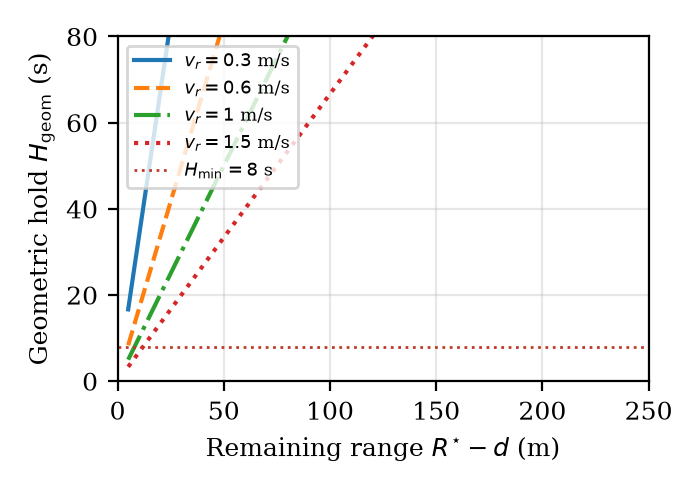
\includegraphics[width=0.92\columnwidth]{figs/hold_time.png}
\caption{Geometric hold time versus remaining range to $R^{\star}$.
The $H_{\min}=8$\,s line is about two in-flight times at $R^{\star}$.}
\label{fig:hold}
\end{figure}

\subsection{Hold-Time-Aware Next Hop}
A next hop $j$ must satisfy $\bar{s}_{ij}\ge\gamma_{\mathrm{th}}$
(table) or $\gamma_{ij}\ge\gamma_{\mathrm{th}}$ (oracle). Relays other
than the sink must reduce range to the USV by at least $40$\,m, using
the last HELLO position. ETHA then applies a hold-time constraint
$H_{ij}\ge H_{\min}=8$\,s (about two in-flight times at $R^{\star}$)
and a depth-primary score toward the surface sink
\begin{equation}
S(j)=
\begin{cases}
10^{6}+\bar{s}_{ij}, & j=0,\\
-z_j+0.02\,\bar{s}_{ij}+0.01\min(H_{ij},120), & j\neq 0.
\end{cases}
\label{eq:score}
\end{equation}
If the filtered set is empty, ETHA falls back to \eqref{eq:score}
without the hold test so a packet is not dropped solely because every
neighbor is fading (Algorithm~\ref{alg:hop}).

Four policies are compared.

\begin{itemize}
\item \textbf{ETHA (proposed).} Event-triggered HELLO, hold filter,
score \eqref{eq:score} on the live table.
\item \textbf{Event/Periodic+SNR.} Maximize $\bar{s}_{ij}$ over the live table.
\item \textbf{Event+Depth.} DBR-like \cite{yan2008dbr}: maximize $-z_j$
among progress-feasible neighbors. This is an ablation of the hold
term in \eqref{eq:score}.
\item \textbf{Oracle.} ETHA score over \emph{all} nodes using true
geometry. The oracle cannot beat physics: a node with no currently
decodable progress neighbor still drops.
\end{itemize}

\begin{algorithm}[!t]
\caption{Table-driven next hop toward sink $d$}
\label{alg:hop}
\begin{algorithmic}[1]
\STATE $\mathcal{N}\leftarrow$ live neighbors of $i$
\STATE $j^{\star}\leftarrow \emptyset$, $\mathrm{best}\leftarrow -\infty$
\FORALL{$j\in\mathcal{N}$}
\STATE require $\bar{s}_{ij}\ge\gamma_{\mathrm{th}}$
\STATE require $j=d$ or geographic progress $\ge 40$\,m
\IF{ETHA \textbf{and} $H_{ij}<H_{\min}$} \STATE \textbf{continue} \ENDIF
\STATE score $\leftarrow S(j)$ in \eqref{eq:score} (ETHA) or $\bar{s}_{ij}$ (SNR) or $-z_j$ (depth)
\IF{$\mathrm{score}>\mathrm{best}$}
\STATE $j^{\star}\leftarrow j$, $\mathrm{best}\leftarrow\mathrm{score}$
\ENDIF
\ENDFOR
\STATE \textbf{if} $j^{\star}=\emptyset$ \textbf{and} ETHA \textbf{then} repeat without the hold test
\STATE \textbf{return} $j^{\star}$ or drop (no-route)
\end{algorithmic}
\end{algorithm}

\subsection{Complexity}
Let $n_i=|\widehat{\mathcal{N}}_i|$. A HELLO decision is $O(1)$:
compare SNR and displacement against $\Delta_s$ and $\Delta_p$.
Updating one neighbor record is $O(1)$ (EWMA plus \eqref{eq:hold}).
A forwarding decision scans the live table once, hence $O(n_i)$,
and $n_i\le N$ with $N\le 15$ in the campaign. There is no Q-table,
no value iteration, and no end-to-end path computation. Memory is
one record per heard neighbor.

\section{Performance Evaluation}
\label{sec:eval}

\subsection{Simulation Settings}
All experiments use NS-3.41 with Aqua-Sim-NG (commit \texttt{0fbc166})
\cite{ns3manual,aquasimng}.
Table~\ref{tab:params} lists the acoustic stack (LQARP Table~II
\cite{liu2026lqarp}). Table~\ref{tab:campaign} lists the two
campaigns. Each seed randomizes placement, thrust, current phase,
current scale, ALOHA backoff, and BPSK erasures. Intervals are
two-sided $95\%$ Student-$t$.

Discovery uses a contour-crossing layout so that true links form and
break inside $240$\,s. Forwarding uses a relay-stable inner ring so
that PDR measures the hop rule rather than a forced partition; data
start at $t=50$\,s after neighbor tables have filled.

\begin{table}[!t]
\caption{Acoustic and MAC Parameters (LQARP Table~II Stack)}
\label{tab:params}
\centering
\begin{tabular}{lc}
\toprule
Parameter & Value \\
\midrule
Carrier $f_{c}$ / bit rate $R_b$ & $24$\,kHz / $1000$\,bit/s \\
Packet length $L$ & $400$\,bit \\
Modulation & BPSK \\
SL / DI & $185$\,dB / $0$\,dB \\
Spreading $k$ & $1.5$ \\
Shipping $s$ / wind $w$ & $0.2$ / $2$\,m/s \\
SNR threshold $\gamma_{\mathrm{th}}$ & $8.68$\,dB \\
Multipath margin $M$ & $30$\,dB ($R^{\star}=4946$\,m) \\
Sound speed $c$ & $1500$\,m/s \\
Transmit power $P_T$ & $10$\,W \\
MAC & unslotted ALOHA, AckOn $=0$ \\
HELLO / data pad & $50$\,B \\
Control budget (reference) & $2$\,kbps \\
\bottomrule
\end{tabular}
\end{table}

\begin{table}[!t]
\caption{Simulation Campaigns}
\label{tab:campaign}
\centering
\resizebox{\columnwidth}{!}{%
\begin{tabular}{lcc}
\toprule
Quantity & Discovery & Forwarding (ETHA) \\
\midrule
Simulator & \multicolumn{2}{c}{NS-3.41 + Aqua-Sim-NG} \\
Nodes & $12$ (contour) & $6$, $12$, $16$ \\
Run length & $240$\,s & $360$\,s \\
Periodic HELLO & $T=5$\,s & $T=5$\,s \\
Event HELLO & $T_{\max}=25$\,s & $T_{\max}=10$\,s \\
Data & --- & every AUV, $8$--$24$\,s, $t\ge 50$\,s \\
Seeds (main) & $30$ & $30$ \\
Seeds (scale / load / appendix) & $20$ & $20$ / $15$ \\
\bottomrule
\end{tabular}}
\end{table}

\subsection{Performance Metrics}
Let $\mathcal{E}(t)$ and $\widehat{\mathcal{E}}(t)$ be the true and
discovered directed-edge sets at snapshot $t$. With
$\mathrm{TP}=|\mathcal{E}\cap\widehat{\mathcal{E}}|$,
$\mathrm{FP}=|\widehat{\mathcal{E}}\setminus\mathcal{E}|$,
$\mathrm{FN}=|\mathcal{E}\setminus\widehat{\mathcal{E}}|$,
\begin{equation}
\mathrm{Prc}=\frac{\mathrm{TP}}{\mathrm{TP}+\mathrm{FP}},\quad
\mathrm{Rec}=\frac{\mathrm{TP}}{\mathrm{TP}+\mathrm{FN}},\quad
F_1=\frac{2\,\mathrm{Prc}\,\mathrm{Rec}}{\mathrm{Prc}+\mathrm{Rec}}.
\label{eq:prf}
\end{equation}
Link-up (link-down) delay is the time from a true edge appearing
(disappearing) until the table agrees. Hold-time MAE is the absolute
error of $H_{ij}$ in the $60$\,s before a true link-down.
Delivery metrics are
\begin{equation}
\mathrm{PDR}=\frac{N_{\mathrm{deliv}}}{N_{\mathrm{orig}}},\qquad
\overline{D}=\frac{1}{N_{\mathrm{deliv}}}\sum (t_{\mathrm{rx}}-t_{\mathrm{tx}}).
\label{eq:pdr}
\end{equation}
Energy is \eqref{eq:energy} counted over HELLO plus data transmissions.
A hop is \emph{stale} if true SNR is already below $\gamma_{\mathrm{th}}$
or true hold is shorter than flight time $d/c+T_{\mathrm{tx}}$, and
\emph{dying} if true hold is below $H_{\min}$.

\subsection{Topology Discovery: Periodic versus Event-Triggered}
\label{sec:disc}
Fig.~\ref{fig:discovery} and Table~\ref{tab:discovery} summarize the
thirty-seed contour-crossing experiment ($T_{\max}=25$\,s).

\begin{figure}[!t]
\centering
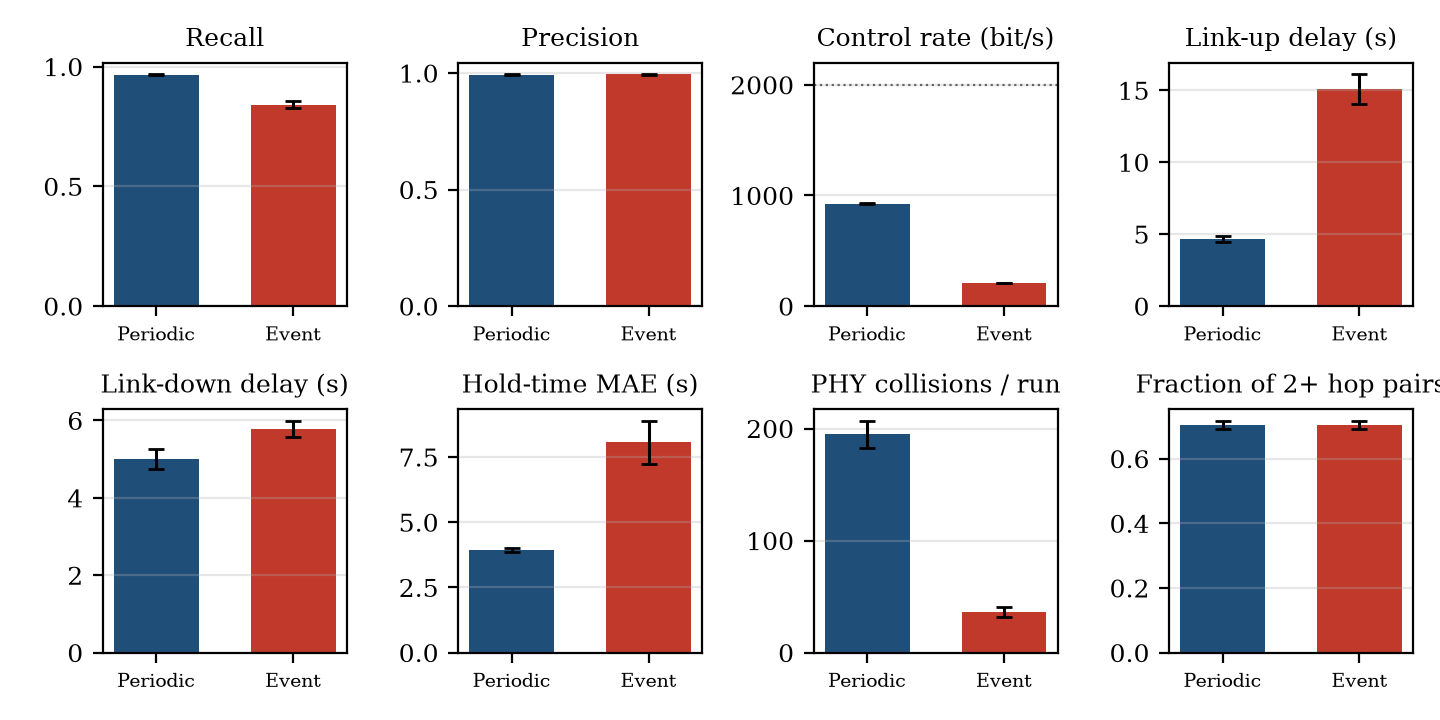
\includegraphics[width=\columnwidth]{figs/discovery_ci.png}
\caption{Discovery metrics, mean and $95\%$ CI over $30$ seeds.
Event-triggered HELLO stays near $11\%$ of a $2$\,kbps budget.
Precision is unchanged; recall, link-up delay, and hold-time MAE pay
for the saved beacons. Link-down delay does not, because the timeout
is SNR-aware.}
\label{fig:discovery}
\end{figure}

\begin{table}[!t]
\caption{Discovery, $30$ Seeds, Mean $\pm$ $95\%$ CI}
\label{tab:discovery}
\centering
\begin{tabular}{lcc}
\toprule
Metric & Periodic & Event \\
\midrule
Recall & $0.966\pm 0.002$ & $0.841\pm 0.015$ \\
Precision & $0.994\pm 0.001$ & $0.994\pm 0.001$ \\
F1 & $0.979\pm 0.001$ & $0.908\pm 0.009$ \\
Control (bit/s) & $927\pm 1$ & $212\pm 1$ \\
Link-up delay (s) & $4.67\pm 0.20$ & $15.1\pm 1.0$ \\
Link-down delay (s) & $5.00\pm 0.26$ & $5.78\pm 0.22$ \\
Hold-time MAE (s) & $3.93\pm 0.07$ & $8.06\pm 0.83$ \\
PHY collisions / run & $195\pm 12$ & $36\pm 4$ \\
$2+$ hop pair fraction & $0.705\pm 0.012$ & $0.705\pm 0.012$ \\
Beacons sent / run & $556\pm 1$ & $127\pm 0.5$ \\
\bottomrule
\end{tabular}
\end{table}

Event-triggered discovery saves about $77\%$ of HELLO transmissions
($O_c=212$ versus $927$\,bit/s) and stays at $11\%$ of the $2$\,kbps
budget. Precision does not move: false neighbors are rare because
decode is SNR-gated after the MAC. The costs are real. Recall drops
by $0.125$. Mean link-up delay grows from $5$\,s to $15$\,s,
consistent with a $25$\,s keep-alive plus ALOHA loss. Hold-time MAE
roughly doubles because the predictor is fed less often.
Link-\emph{down} delay does not inflate, which is \eqref{eq:timeout}:
a fading EWMA is declared dead in about $6$\,s rather than
$3T_{\max}=75$\,s. Every seed produced $5$--$14$ true link-down
events; the delays are not a two-event anecdote.

PHY collisions fall from $195$ to $36$ per run. That is a second
budget: fewer HELLOs leave airtime for data. It is also why a
learning router that ignores the HELLO process will mis-attribute
collisions.

\subsection{Impact of Keep-Alive, Slotting, Margin, and Scale}
\label{sec:ablate}
Fig.~\ref{fig:tmax} and Table~\ref{tab:tmax} sweep $T_{\max}$ at
$n=20$ seeds. Stretching the keep-alive past $25$\,s does not buy
recall; it only stale-dates hold time (MAE $13.9$\,s at
$T_{\max}=40$\,s). $T_{\max}=10$\,s recovers recall $0.883$ and
hold MAE $4.85$\,s at $488$\,bit/s---still a quarter of a $2$\,kbps
budget, and the awareness-friendly operating point used for
forwarding. $T_{\max}=25$\,s is the budget-friendly discovery point.

\begin{figure}[!t]
\centering
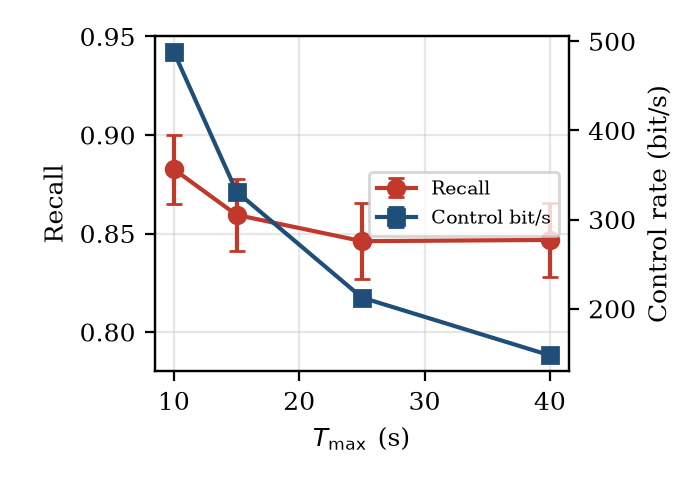
\includegraphics[width=0.92\columnwidth]{figs/tmax_tradeoff.png}
\caption{Event-triggered keep-alive sweep (unslotted ALOHA, $12$ nodes,
$n=20$). Recall saturates; control rate and hold-time error do not.}
\label{fig:tmax}
\end{figure}

\begin{table}[!t]
\caption{Event-Triggered $T_{\max}$ Sweep ($n=20$)}
\label{tab:tmax}
\centering
\begin{tabular}{cccc}
\toprule
$T_{\max}$ (s) & Recall & Control (bit/s) & Hold MAE (s) \\
\midrule
$10$ & $0.883\pm 0.018$ & $488\pm 0.3$ & $4.85\pm 0.13$ \\
$15$ & $0.859\pm 0.018$ & $331\pm 0.7$ & $5.55\pm 0.28$ \\
$25$ & $0.846\pm 0.019$ & $213\pm 1$ & $7.90\pm 0.98$ \\
$40$ & $0.847\pm 0.019$ & $148\pm 1$ & $13.9\pm 1.9$ \\
\bottomrule
\end{tabular}
\end{table}

Slotted ALOHA is worse in this geometry, not better. A UWA slot of
$5.06$\,s lines up with the $5$\,s HELLO period. Periodic slotted
recall falls to $0.818$ and collisions rise to $477$ per run.
We keep unslotted ALOHA as the main MAC and report slotted as a
negative control.

Multipath margin $M\in\{20,30,40\}$\,dB rescales
$R^{\star}\in\{6407,4946,3564\}$\,m. Because nodes are placed as
fractions of $R^{\star}$, recall, edge count, and the two-hop fraction
do not change in any operationally meaningful way. This is a
sensitivity check, not a substitute for Bellhop.

Node count matters for discovery. A $6$-node ring is a near-clique
($2+$ hop fraction $0.26$, diameter $1.47$). Event-triggered recall
collapses to $0.59$ because everyone sits on the $R^{\star}$ contour
and send-on-delta rarely fires. Twelve and sixteen nodes both have a
$2+$ hop fraction near $0.70$ and event recall $0.85$--$0.86$.
We quote $12$ nodes as the operating point and do not quote the
six-node clique as evidence of a protocol.

\subsection{Packet Delivery Ratio}
\label{sec:pdr}
All AUVs originate $400$-bit packets every $16$\,s after $t=50$\,s
on the relay-stable inner/outer field, $T_{\max}=10$\,s, $360$\,s,
$n=30$. Fig.~\ref{fig:fwd} and Table~\ref{tab:fwd} are the main
comparison.

\begin{figure*}[!t]
\centering
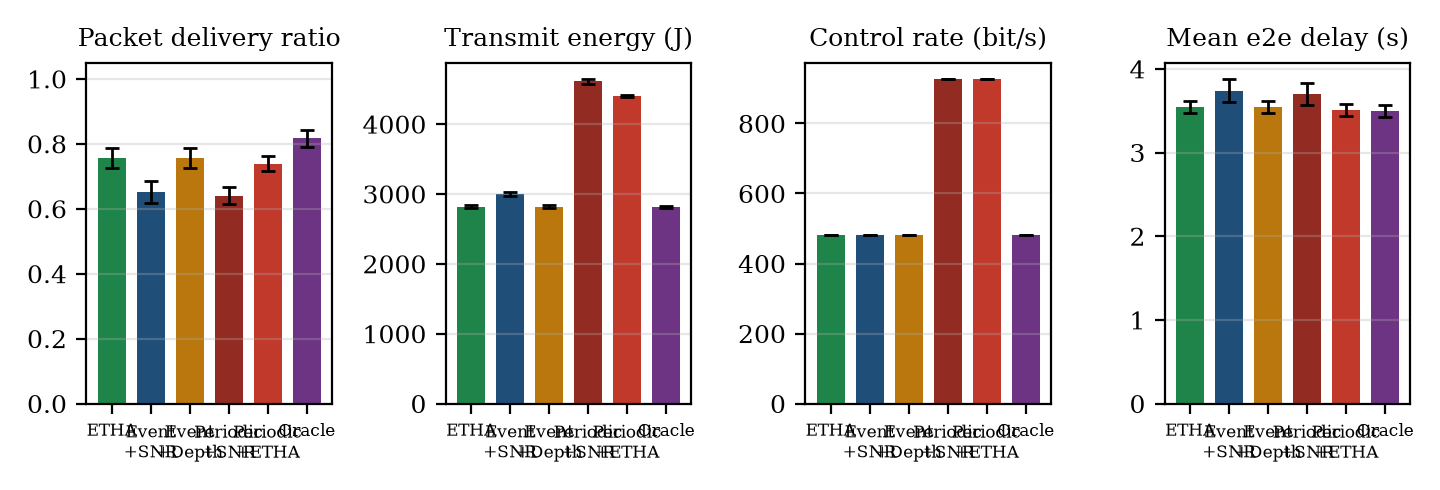
\includegraphics[width=0.92\textwidth]{figs/forwarding_ci.png}
\caption{Forwarding campaign, $12$ nodes, $n=30$, $95\%$ CI.
ETHA matches a DBR-like depth baseline on PDR and delay while cutting
transmit energy and HELLO rate relative to periodic SNR-greedy
forwarding. Oracle is an upper bound with perfect geometry, not a protocol.}
\label{fig:fwd}
\end{figure*}

\begin{table}[!t]
\caption{Forwarding, $12$ Nodes, Mean $\pm$ $95\%$ CI ($n=30$)}
\label{tab:fwd}
\centering
\small
\setlength{\tabcolsep}{2.0pt}
\resizebox{\columnwidth}{!}{%
\begin{tabular}{lccccc}
\toprule
Scheme & PDR & $E_{\mathrm{tx}}$ (kJ) & $O_c$ & Delay (s) & No-route \\
\midrule
ETHA (proposed) & $0.755\pm 0.031$ & $2.82\pm 0.02$ & $480$ & $3.54\pm 0.07$ & $12.7\pm 6.1$ \\
Event+SNR & $0.651\pm 0.033$ & $3.00\pm 0.03$ & $480$ & $3.74\pm 0.14$ & $14.5\pm 7.0$ \\
Event+Depth & $0.755\pm 0.031$ & $2.82\pm 0.02$ & $480$ & $3.54\pm 0.07$ & $12.7\pm 6.1$ \\
Periodic+SNR & $0.641\pm 0.027$ & $4.61\pm 0.03$ & $927$ & $3.70\pm 0.13$ & $2.07\pm 1.2$ \\
Periodic+ETHA & $0.739\pm 0.023$ & $4.41\pm 0.02$ & $926$ & $3.51\pm 0.07$ & $1.53\pm 0.71$ \\
Oracle & $0.817\pm 0.027$ & $2.81\pm 0.02$ & $480$ & $3.50\pm 0.07$ & $0$ \\
\bottomrule
\end{tabular}}
\end{table}

ETHA delivers $\mathrm{PDR}=0.755$, a $18\%$ relative gain over
periodic SNR-greedy ($0.641$) and a $16\%$ gain over event SNR-greedy
($0.651$) on the same event map. Mean hop count falls from $1.66$
(SNR-greedy) to $1.37$ (ETHA): depth-primary scoring walks toward the
surface rather than toward a deep, high-SNR neighbor that is a
geographic dead end. Stale in-flight hops are zero.

Event+Depth matches ETHA on every delivery statistic to the reported
precision. That is a measured fact, not a hidden claim. On this
relay-stable field the hold filter rarely binds ($H_{\min}=8$\,s,
inner AUVs well inside $R^{\star}$), so \eqref{eq:score} reduces to
a DBR-like rule plus a vanishing SNR/hold tie-break. ETHA is not
proposed as a replacement for depth when the sink is the surface; it
is proposed as the way to \emph{afford} that hop rule, by not spending
$927$\,bit/s on HELLOs, and as the filter that would bind if the
contour were crossed in flight.

The oracle with perfect geometry reaches $0.817$ at the same event
HELLO rate, with zero no-route. ETHA's remaining $0.062$ of PDR is
the $12.7$ no-route drops per run from table holes, not hop scoring.
Periodic HELLO almost eliminates no-route ($2.07$) but does not
translate that map density into PDR under SNR-greedy scoring, because
the extra $447$\,bit/s of HELLO also raise PHY collisions from $336$
to $629$ per run. Periodic+ETHA ($0.739$) is close to event ETHA
($0.755$) at $56\%$ more transmit energy: once the scorer is
depth-primary, further HELLOs buy little delivery and cost a great
deal of airtime.

\subsection{Energy Consumption}
Transmit energy follows \eqref{eq:energy}. ETHA spends $2.82$\,kJ per
$360$\,s run versus $4.61$\,kJ for periodic SNR-greedy: a $39\%$
saving. Table~\ref{tab:edec} splits that total into HELLO and data.
Event schemes emit $432$ HELLOs ($480$\,bit/s), hence $1.73$\,kJ of
beacon energy; periodic schemes emit about $834$ HELLOs, hence
$3.34$\,kJ. The remaining $1.09$\,kJ (ETHA) versus $1.28$\,kJ
(periodic SNR-greedy) is data origination and forwarding. ETHA's
shorter paths therefore save a further $0.19$\,kJ on top of the
$1.61$\,kJ HELLO saving. Event+SNR sits at $3.00$\,kJ total; the extra
$0.18$\,kJ relative to ETHA is additional data forwards on longer
SNR-greedy paths, not extra HELLOs. Periodic+ETHA ($4.41$\,kJ) shows
that rewriting the hop score without rewriting HELLO still leaves
about $1.6$\,kJ on the table.
Fig.~\ref{fig:scale} (right) confirms the gap at every node count:
at $16$ nodes ETHA uses $3.93$\,kJ against $6.31$\,kJ for periodic
SNR-greedy.

\begin{table}[!t]
\caption{Transmit-Energy Decomposition, $12$ Nodes, $360$\,s}
\label{tab:edec}
\centering
\begin{tabular}{lccc}
\toprule
Scheme & HELLO (kJ) & Data (kJ) & Total (kJ) \\
\midrule
ETHA & $1.73$ & $1.09$ & $2.82$ \\
Event+SNR & $1.73$ & $1.27$ & $3.00$ \\
Periodic+SNR & $3.34$ & $1.28$ & $4.61$ \\
Periodic+ETHA & $3.34$ & $1.07$ & $4.41$ \\
\bottomrule
\end{tabular}
\end{table}

\subsection{End-to-End Delay and Hop Count}
Mean e2e delay is one acoustic flight plus a short contention:
$3.54$\,s for ETHA versus $3.74$\,s for event SNR-greedy and
$3.70$\,s for periodic SNR-greedy. The differences are tens of
milliseconds of extra hops and ALOHA backoff, not a routing-layer
queue. Hop count $1.37$ versus $1.66$ is the geographic content of
\eqref{eq:score}: more packets reach the USV in one hop because the
scorer prefers the surface.
Fig.~\ref{fig:scale} (bottom) repeats delay and hop count against
node count: both rise with load, and ETHA stays below periodic
SNR-greedy at every scale because it takes shorter surface-seeking
paths.

\subsection{Control Overhead}
HELLO rate is deterministic in this campaign once $T_{\max}$ and $T$
are fixed: $480$\,bit/s for every event scheme ($T_{\max}=10$\,s) and
$927$\,bit/s for every periodic scheme ($T=5$\,s), against a
$2$\,kbps reference. ETHA therefore occupies $24\%$ of the control
budget where periodic occupies $46\%$. Combined with
Section~\ref{sec:disc}, the operator has two documented points:
$T_{\max}=25$\,s at $11\%$ of budget for awareness, and
$T_{\max}=10$\,s at $24\%$ of budget for forwarding.

\subsection{Scalability}
Fig.~\ref{fig:scale} and Table~\ref{tab:scale} scale the network at
the same per-AUV load (one $400$-bit packet every $16$\,s).
PDR falls with node count for every scheme, as expected under
unslotted ALOHA \cite{casari2011protocol}. ETHA stays above periodic
SNR-greedy at $6$, $12$, and $16$ nodes
($0.875$, $0.755$, $0.657$ versus $0.865$, $0.641$, $0.525$).
The gap widens as collisions grow: at $16$ nodes ETHA's HELLO rate is
$640$\,bit/s versus $1236$\,bit/s periodic, and PDR is $0.13$ higher.
Six-node graphs are a dense reference; they are not the operating
point we quote in the abstract.

\begin{figure*}[!t]
\centering
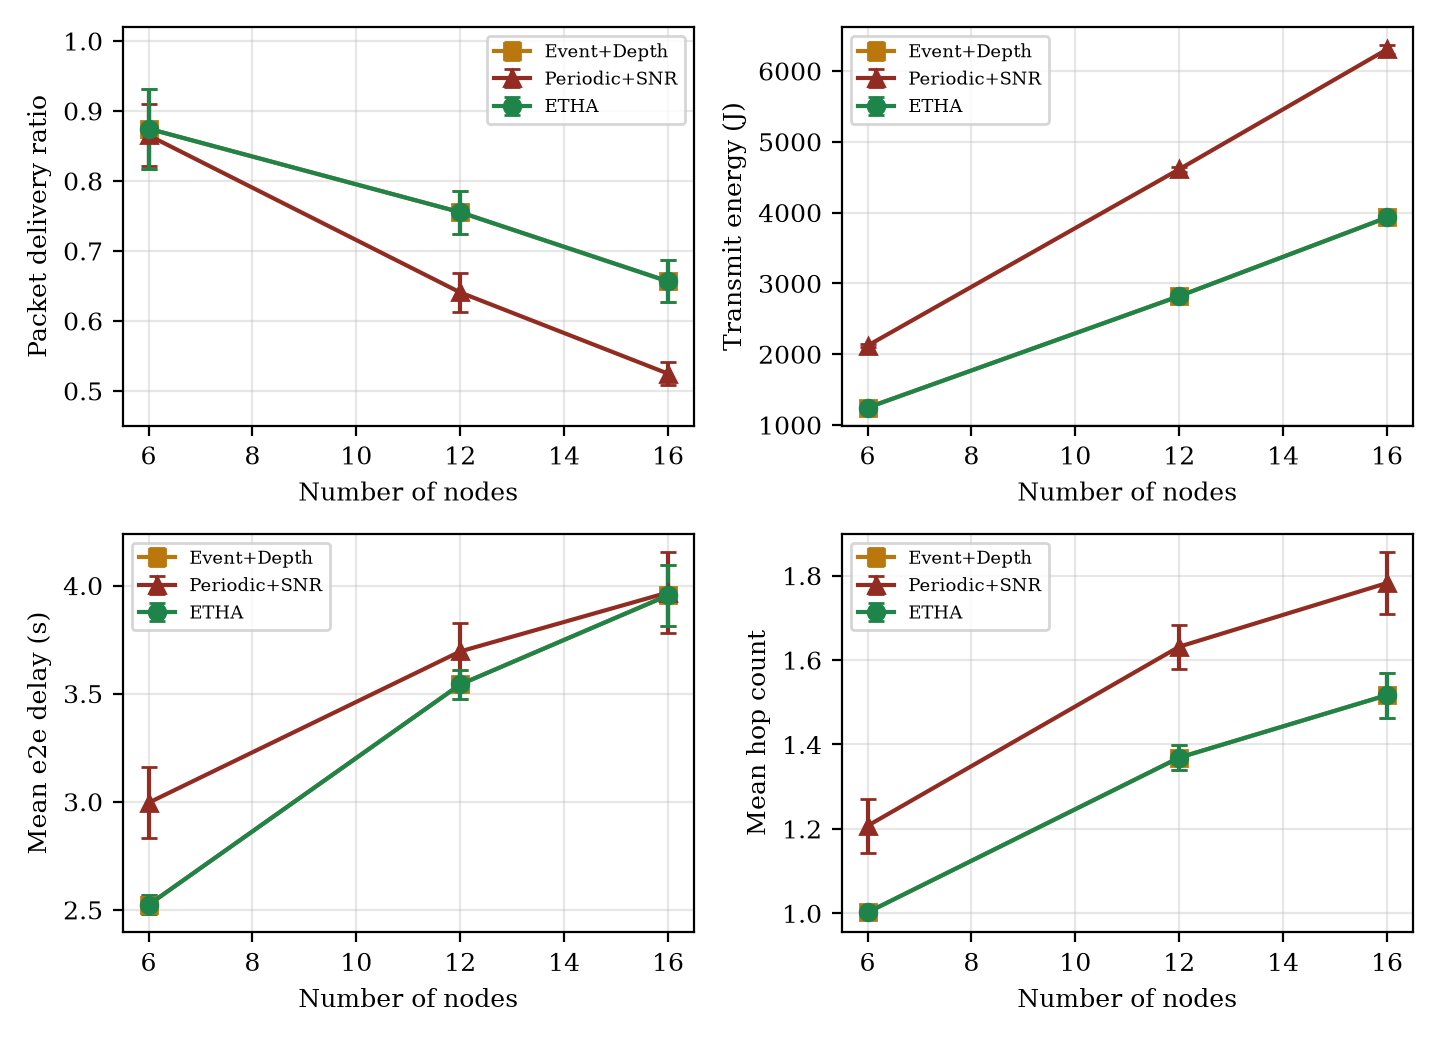
\includegraphics[width=0.98\textwidth]{figs/pdr_vs_nodes.png}
\caption{LQARP-style scale plots ($95\%$ CI): packet delivery ratio,
transmit energy, end-to-end delay, and hop count versus number of
nodes. Load is one $400$-bit packet per AUV per $16$\,s. ETHA and
Event+Depth coincide on this field (hold rarely binds).}
\label{fig:scale}
\end{figure*}

\begin{table}[!t]
\caption{PDR and Energy versus Node Count, Mean $\pm$ $95\%$ CI}
\label{tab:scale}
\centering
\setlength{\tabcolsep}{3pt}
\begin{tabular}{lcccccc}
\toprule
 & \multicolumn{2}{c}{ETHA} & \multicolumn{2}{c}{Event+Depth} & \multicolumn{2}{c}{Periodic+SNR} \\
\cmidrule(lr){2-3}\cmidrule(lr){4-5}\cmidrule(lr){6-7}
Nodes & PDR & $E$ (kJ) & PDR & $E$ (kJ) & PDR & $E$ (kJ) \\
\midrule
$6$ ($n=20$) & $0.875$ & $1.25$ & $0.875$ & $1.25$ & $0.865$ & $2.12$ \\
$12$ ($n=30$) & $0.755$ & $2.82$ & $0.755$ & $2.82$ & $0.641$ & $4.61$ \\
$16$ ($n=20$) & $0.657$ & $3.93$ & $0.657$ & $3.93$ & $0.525$ & $6.31$ \\
\bottomrule
\end{tabular}
\end{table}

\subsection{Impact of Traffic Load}
Fig.~\ref{fig:load} and Table~\ref{tab:load} vary the packet
generation interval in $\{8,12,16,24\}$\,s at $12$ nodes
($n=15$ except $n=30$ at $16$\,s). ETHA PDR is essentially flat
($0.746$--$0.755$): at these offered loads the pipe is not saturated,
and the first-order residual remains next-hop geography plus table
holes. Periodic SNR-greedy stays $0.12$--$0.14$ below ETHA at every
interval and spends $1.7$--$2.0$\,kJ more. Tightening the interval
from $24$\,s to $8$\,s raises ETHA energy from $2.47$\,kJ to
$3.88$\,kJ because more data packets are originated and forwarded;
the HELLO component does not change. Fig.~\ref{fig:load} also reports
delay and control rate versus interval: delay is insensitive to load
in this regime, and HELLO overhead does not grow with data rate
because beacons are event-triggered, not piggybacked.

\begin{figure*}[!t]
\centering
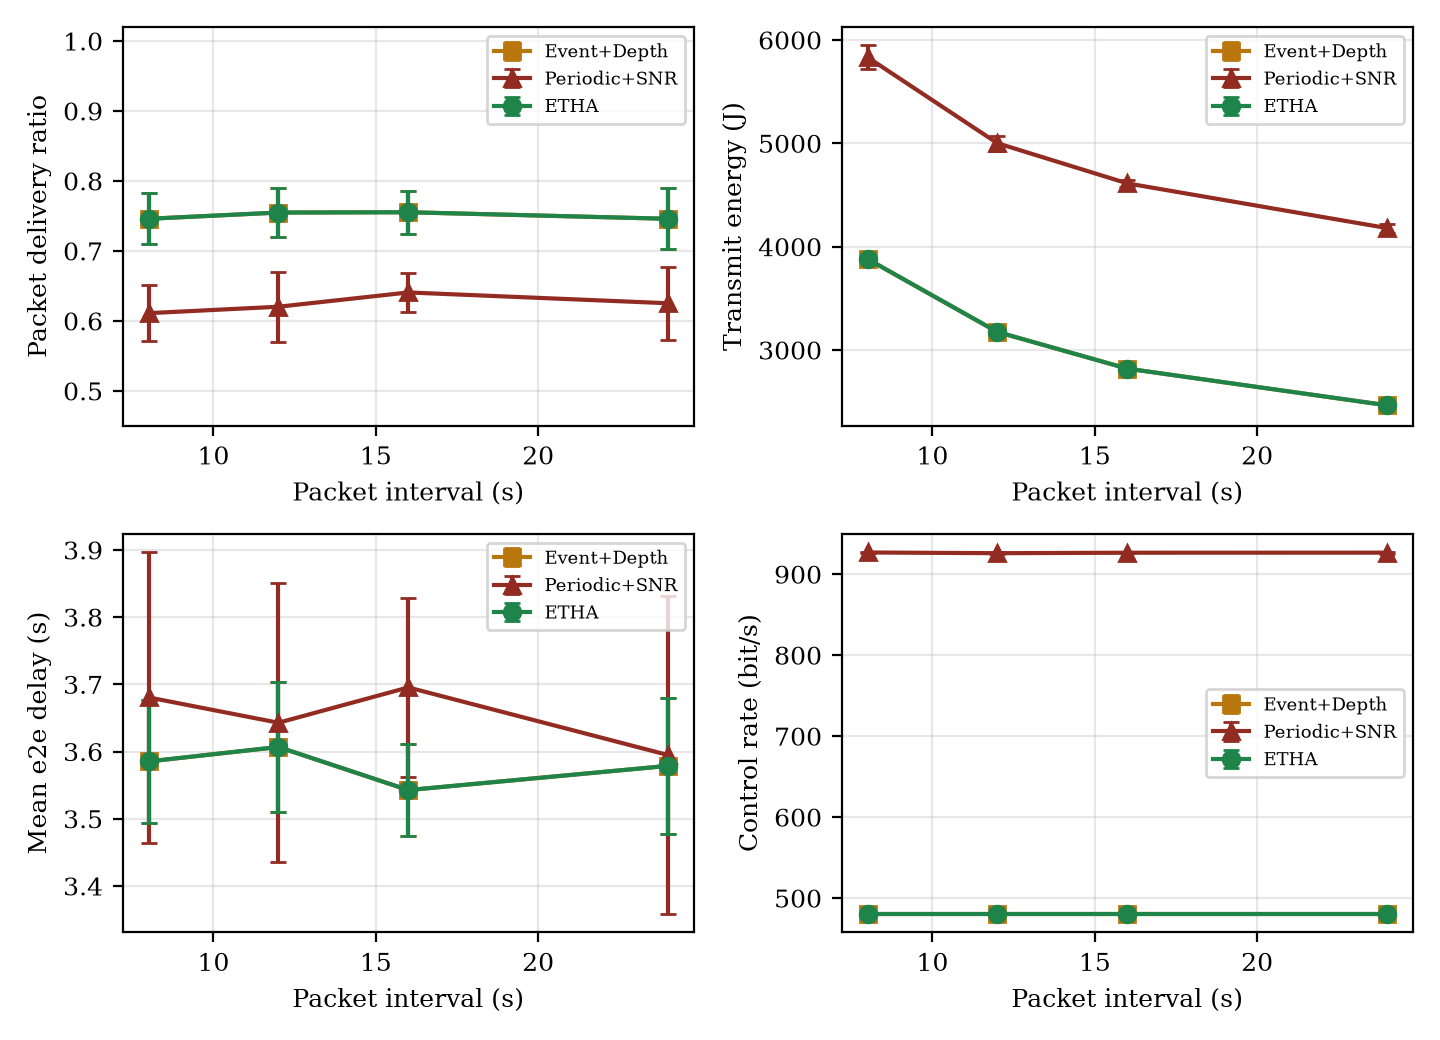
\includegraphics[width=0.98\textwidth]{figs/load_tradeoff.png}
\caption{LQARP-style load plots ($95\%$ CI): PDR, transmit energy,
end-to-end delay, and HELLO control rate versus packet generation
interval at $12$ nodes.}
\label{fig:load}
\end{figure*}

\begin{table}[!t]
\caption{PDR versus Packet Interval, $12$ Nodes}
\label{tab:load}
\centering
\begin{tabular}{lccc}
\toprule
Interval (s) & ETHA & Event+Depth & Periodic+SNR \\
\midrule
$8$ ($n=15$) & $0.746\pm 0.037$ & $0.746\pm 0.037$ & $0.611\pm 0.040$ \\
$12$ ($n=15$) & $0.755\pm 0.035$ & $0.755\pm 0.035$ & $0.620\pm 0.050$ \\
$16$ ($n=30$) & $0.755\pm 0.031$ & $0.755\pm 0.031$ & $0.641\pm 0.027$ \\
$24$ ($n=15$) & $0.746\pm 0.044$ & $0.746\pm 0.044$ & $0.625\pm 0.052$ \\
\bottomrule
\end{tabular}
\end{table}

\subsection{Discussion and Limitations}
The first-order residual on a mobile USV--AUV acoustic pipe is the
HELLO budget together with next-hop geography, not a learned Q-table.
Event-triggered discovery at $T_{\max}=10$\,s buys a neighbor table
that is good enough for $\mathrm{PDR}=0.755$ at $12$ nodes while
leaving more than $1.6$\,kJ and $447$\,bit/s on the table relative to
periodic SNR-greedy HELLO. Hold-time-aware scoring is the correct
filter when links die in flight; on the relay-stable forwarding field
those events are rare, ETHA coincides with Event+Depth, and the paper
reports that coincidence. Depth-greedy remains available as a hop
rule on top of ETHA's map. Q-learning in the style of LQARP
\cite{liu2026lqarp,hu2010qelar} is the natural sequel once the
map---not the scorer---is the residual that remains, and only among
neighbors the node has actually heard.

The link model is analytical. There is no Bellhop TL table, no
measured CSI, and no sea trial. Hold time is kinematic. Forwarding is
single-path. Receive energy is not counted. The layout is engineered
so that $R^{\star}$ is meaningful; a field whose nodes never approach
the contour would show fewer link-down events and a weaker hold-time
story. Those limits are why the claims stop at discovery plus a
transparent hop filter.

\section{Conclusion}
\label{sec:concl}
This paper wrote the missing first chapter of a mobile USV--AUV
acoustic network that must live inside $2$\,kbps of control traffic.
Section~\ref{sec:prelim} defined the architecture, the
Urick--Thorp--Wenz channel, the constant-margin treatment of
multipath, and the Q-learning loop that LQARP trains---without
training it.
The system model instantiates that channel as
\eqref{eq:thorp}--\eqref{eq:energy} in Aqua-Sim-NG.
Event-triggered HELLO at $T_{\max}=25$\,s cuts discovery overhead from
$927$ to $212$\,bit/s at a measured cost in recall. The forwarding
operating point $T_{\max}=10$\,s, together with hold-time-aware
depth-primary next-hop selection (ETHA), raises PDR from $0.641$
(periodic SNR-greedy) to $0.755$ at $12$ nodes ($n=30$) while cutting
transmit energy from $4.61$\,kJ to $2.82$\,kJ and HELLO traffic from
$927$ to $480$\,bit/s. A DBR-like depth ablation on the same map
matches ETHA and is reported as a baseline, not hidden. An oracle
bound of $0.817$ locates the remaining gap in missing relays.
The next chapter is a learner that is only allowed to choose among
neighbors ETHA has actually heard.

\section*{Acknowledgment}
The author thanks the Aqua-Sim-NG and ns-3 maintainers. Simulation
code and seed-level traces for this manuscript live in the companion
repository.

\begin{thebibliography}{00}

\bibitem{akyildiz2005uasn}
I.~F. Akyildiz, D.~Pompili, and T.~Melodia, ``Underwater acoustic sensor networks: Research challenges,'' \emph{Ad Hoc Netw.}, vol.~3, no.~3, pp.~257--279, 2005.

\bibitem{sozer2000uan}
E.~M. Sozer, M.~Stojanovic, and J.~G. Proakis, ``Underwater acoustic networks,'' \emph{{IEEE} J. Ocean. Eng.}, vol.~25, no.~1, pp.~72--83, 2000.

\bibitem{stojanovic2007capacity}
M.~Stojanovic, ``On the relationship between capacity and distance in an underwater acoustic communication channel,'' \emph{{ACM} {SIGMOBILE} Mobile Comput. Commun. Rev.}, vol.~11, no.~4, pp.~34--43, 2007.

\bibitem{stojanovic2009channels}
M.~Stojanovic and J.~Preisig, ``Underwater acoustic communication channels: Propagation models and statistical characterization,'' \emph{{IEEE} Commun. Mag.}, vol.~47, no.~1, pp.~84--89, 2009.

\bibitem{urick1983sound}
R.~J. Urick, \emph{Principles of Underwater Sound}, 3rd~ed. Peninsula Publishing, 1983.

\bibitem{thorp1967attenuation}
W.~H. Thorp, ``Analytic description of the low-frequency attenuation coefficient,'' \emph{J. Acoust. Soc. Amer.}, vol.~42, no.~1, p.~270, 1967.

\bibitem{wenz1962noise}
G.~M. Wenz, ``Acoustic ambient noise in the ocean: Spectra and sources,'' \emph{J. Acoust. Soc. Amer.}, vol.~34, no.~12, pp.~1936--1956, 1962.

\bibitem{caruso2008mcm}
A.~Caruso, F.~Paparella, L.~F.~M. Vieira, M.~Erol, and M.~Gerla, ``The meandering current mobility model and its impact on underwater mobile sensor networks,'' in \emph{Proc. {IEEE} INFOCOM}, 2008, pp.~221--225.

\bibitem{heemels2012event}
W.~P.~M.~H. Heemels, K.~H. Johansson, and P.~Tabuada, ``An introduction to event-triggered and self-triggered control,'' in \emph{Proc. {IEEE} CDC}, 2012, pp.~3270--3285.

\bibitem{tabuada2007event}
P.~Tabuada, ``Event-triggered real-time scheduling of stabilizing control tasks,'' \emph{{IEEE} Trans. Autom. Control}, vol.~52, no.~9, pp.~1680--1685, 2007.

\bibitem{watkins1992qlearning}
C.~J.~C.~H. Watkins and P.~Dayan, ``{Q}-learning,'' \emph{Mach. Learn.}, vol.~8, nos.~3--4, pp.~279--292, 1992.

\bibitem{sutton2018rl}
R.~S. Sutton and A.~G. Barto, \emph{Reinforcement Learning: An Introduction}, 2nd~ed. MIT Press, 2018.

\bibitem{xie2006vbf}
P.~Xie, J.-H. Cui, and L.~Lao, ``{VBF}: Vector-based forwarding protocol for underwater sensor networks,'' in \emph{Proc. IFIP Networking}, 2006, pp.~1216--1221.

\bibitem{yan2008dbr}
H.~Yan, Z.~J. Shi, and J.-H. Cui, ``{DBR}: Depth-based routing for underwater sensor networks,'' in \emph{Proc. WASA}, 2008, pp.~72--86.

\bibitem{nicolaou2007hhvbf}
N.~Nicolaou, A.~See, P.~Xie, J.-H. Cui, and D.~Maggiorini, ``Improving the robustness of location-based routing for underwater sensor networks,'' in \emph{Proc. OCEANS}, 2007.

\bibitem{hu2010qelar}
T.~Hu and Y.~Fei, ``{QELAR}: A machine-learning-based adaptive routing protocol for energy-efficient and lifetime-extended underwater sensor networks,'' \emph{{IEEE} Trans. Mobile Comput.}, vol.~9, no.~6, pp.~796--809, 2010.

\bibitem{liu2026lqarp}
J.~Liu \emph{et al.}, ``{LQARP}: A link-quality-aware {Q}-learning routing protocol for underwater acoustic sensor networks,'' \emph{{IEEE} Internet of Things J.}, 2026, early access. Acoustic stack and Table~II parameters are the baseline of this work.

\bibitem{xie2009aquasim}
P.~Xie \emph{et al.}, ``Aqua-{Sim}: An {NS}-2 based simulator for underwater sensor networks,'' in \emph{Proc. MTS/{IEEE} OCEANS}, 2009.

\bibitem{casari2011protocol}
P.~Casari and M.~Zorzi, ``Protocol design issues in underwater acoustic networks,'' \emph{Comput. Commun.}, vol.~34, no.~17, pp.~2013--2025, 2011.

\bibitem{chitre2008uwa}
M.~Chitre, S.~Shahabudeen, and M.~Stojanovic, ``Underwater acoustic communications and networking: Recent advances and future challenges,'' \emph{Marine Technol. Soc. J.}, vol.~42, no.~1, pp.~103--116, 2008.

\bibitem{heidemann2012uwsns}
J.~Heidemann, M.~Stojanovic, and M.~Zorzi, ``Underwater sensor networks: applications, advances and challenges,'' \emph{Philos. Trans. Roy. Soc. A}, vol.~370, no.~1958, pp.~158--175, 2012.

\bibitem{preisig2007propagation}
J.~Preisig, ``Acoustic propagation considerations for underwater acoustic communications network development,'' \emph{{ACM} {SIGMOBILE} Mobile Comput. Commun. Rev.}, vol.~11, no.~4, pp.~2--10, 2007.

\bibitem{vanwalree2013scattering}
P.~A. van~Walree, ``Propagation and scattering effects in underwater acoustic communication channels,'' \emph{{IEEE} J. Ocean. Eng.}, vol.~38, no.~4, pp.~632--640, 2013.

\bibitem{coutinho2014gedar}
R.~W.~L. Coutinho, A.~Boukerche, L.~F.~M. Vieira, and A.~A.~F. Loureiro, ``{GEDAR}: Geographic and opportunistic routing protocol with depth adjustment for mobile underwater sensor networks,'' in \emph{Proc. {IEEE} ICC}, 2014, pp.~251--256.

\bibitem{noh2013vapr}
Y.~Noh, U.~Lee, P.~Wang, B.~S. Choi, and M.~Gerla, ``{VAPR}: Void-aware pressure routing for underwater sensor networks,'' \emph{{IEEE} Trans. Mobile Comput.}, vol.~12, no.~5, pp.~895--908, 2013.

\bibitem{akyildiz2007state}
I.~F. Akyildiz, D.~Pompili, and T.~Melodia, ``State-of-the-art in protocol research for underwater acoustic sensor networks,'' \emph{{ACM} {SIGMOBILE} Mobile Comput. Commun. Rev.}, vol.~11, no.~4, pp.~11--22, 2007.

\bibitem{porter2011bellhop}
M.~B. Porter, ``The {BELLHOP} manual and user's guide,'' Heat, Light, and Sound Research, Inc., Tech. Rep., 2011.

\bibitem{woo2003taming}
A.~Woo, T.~Tong, and D.~Culler, ``Taming the underlying challenges of reliable multihop routing in sensor networks,'' in \emph{Proc. {ACM} SenSys}, 2003, pp.~14--27.

\bibitem{fonseca2007fourbit}
R.~Fonseca, O.~Gnawali, K.~Jamieson, and P.~Levis, ``Four-bit wireless link estimation,'' in \emph{Proc. HotNets}, 2007.

\bibitem{ns3manual}
ns-3 Project, \emph{ns-3 Network Simulator, Release 3.41}, 2024. [Online]. Available: \url{https://www.nsnam.org}

\bibitem{aquasimng}
R.~Martin \emph{et al.}, ``Aqua-{Sim} {NG}: Next generation underwater network simulator,'' Univ. of Connecticut, 2024. [Online]. Available: \url{https://github.com/rmartin5/aqua-sim-ng}

\end{thebibliography}

\begin{IEEEbiographynophoto}{Ghulam Ali}
is the corresponding author. E-mail: ghulamali.cs@gmail.com.
His current work concerns topology discovery, link-quality assessment,
and hold-time-aware forwarding for mobile USV--AUV acoustic networks,
with simulation on Aqua-Sim-NG and NS-3.
\end{IEEEbiographynophoto}

\end{document}
